% =====================================================================
%  SMA Place Finder -- Software Stack Documentation
%
%  Build:  tectonic -X compile software_stack_documentation.tex
%     or:  latexmk -pdf software_stack_documentation.tex
%
%  Every technology, version and component in this document was read out
%  of the repository. Anything that could not be verified is marked.
% =====================================================================
\documentclass[11pt,a4paper]{report}

\usepackage[T1]{fontenc}
\usepackage[utf8]{inputenc}
\usepackage{lmodern}
\usepackage[english]{babel}
\usepackage[a4paper,margin=2.4cm,headheight=14pt]{geometry}
\usepackage{graphicx}
\usepackage{xcolor}
\usepackage{booktabs}
\usepackage{longtable}
\usepackage{tabularx}
\usepackage{array}
\usepackage{float}
\usepackage{enumitem}
\usepackage{fancyhdr}
\usepackage{amsmath}
\usepackage{tikz}
\usepackage{pdflscape}
\usepackage{caption}
\usepackage[hidelinks,bookmarksnumbered]{hyperref}
\usepackage{bookmark}

\usetikzlibrary{positioning,shapes.geometric,arrows.meta,calc,fit,backgrounds}

% ---------------------------------------------------------------- colours
\definecolor{cFront}{HTML}{1F6FB2}   % frontend
\definecolor{cBack}{HTML}{1E7A46}    % backend
\definecolor{cData}{HTML}{B5651D}    % storage
\definecolor{cExt}{HTML}{6B6B6B}     % external services
\definecolor{cInfra}{HTML}{6A4C93}   % build / packaging
\definecolor{cNote}{HTML}{8A8A8A}
\definecolor{cRule}{HTML}{1F4E79}
\definecolor{cSoft}{HTML}{F2F6FA}

% ---------------------------------------------------------------- styling
\pagestyle{fancy}
\fancyhf{}
\fancyhead[L]{\footnotesize SMA Place Finder}
\fancyhead[R]{\footnotesize Software Stack Documentation}
\fancyfoot[C]{\thepage}
\renewcommand{\headrulewidth}{0.4pt}

\captionsetup{font=small,labelfont=bf}
\setlength{\emergencystretch}{3em}
\sloppy
\setlist{nosep,leftmargin=1.4em}

\newcommand{\code}[1]{\texttt{\small #1}}
\urlstyle{tt}
% Paths must be able to wrap: in a narrow table column an unbreakable path is
% the one thing that pushes text past the margin.
\DeclareRobustCommand{\file}[1]{{\small\nolinkurl{#1}}}
\newcommand{\ver}[1]{\texttt{#1}}
\newcommand{\nv}{\textcolor{cNote}{\textit{Not Verified}}}
\newcommand{\na}{\textcolor{cNote}{\textit{N/A}}}

% Verification labels used throughout
\newcommand{\lblV}{\textcolor{cBack}{\textbf{Verified}}}
\newcommand{\lblD}{\textcolor{cFront}{\textbf{Derived}}}
\newcommand{\lblR}{\textcolor{cInfra}{\textbf{Recommended}}}
\newcommand{\lblU}{\textcolor{cNote}{\textbf{Unknown}}}

% TikZ node styles
\tikzset{
  box/.style   = {rectangle, rounded corners=2pt, draw=#1, fill=#1!6, text=black,
                  align=center, minimum height=9mm, inner xsep=4pt, font=\scriptsize},
  proc/.style  = {rectangle, rounded corners=5pt, draw=cBack, fill=cBack!6,
                  align=center, minimum height=8mm, font=\scriptsize},
  dec/.style   = {diamond, aspect=2.1, draw=cData, fill=cData!8,
                  align=center, inner sep=1pt, font=\scriptsize},
  db/.style    = {cylinder, shape border rotate=90, aspect=0.25, draw=cData,
                  fill=cData!8, align=center, minimum height=10mm, font=\scriptsize},
  ext/.style   = {rectangle, draw=cExt, fill=cExt!8, dashed, align=center,
                  minimum height=8mm, font=\scriptsize},
  term/.style  = {ellipse, draw=cBack, fill=cBack!8, align=center, font=\scriptsize},
  fl/.style    = {-{Stealth[length=2mm]}, thick, draw=#1},
  flo/.style   = {-{Stealth[length=2mm]}, thick, dashed, draw=cNote},
  lbl/.style   = {font=\tiny, inner sep=1.5pt, fill=white},
}

\begin{document}

% =====================================================================
\begin{titlepage}
\centering
\vspace*{1.2cm}
{\color{cRule}\rule{\textwidth}{1.6pt}}\\[0.5cm]
{\Huge\bfseries SMA Place Finder\par}
\vspace{0.35cm}
{\LARGE Software Stack Documentation\par}
\vspace{0.3cm}
{\color{cRule}\rule{\textwidth}{1.6pt}}\\[1.1cm]

\begin{minipage}{0.84\textwidth}
\centering
\large
\begin{tabular}{@{}ll@{}}
\textbf{Repository}        & \code{atlas-place-finder}\\
\textbf{Application version} & \ver{1.0.0}\ \ \footnotesize(\file{package.json}, \file{tauri.conf.json})\\
\textbf{Documented commit} & \code{cfb509b} (2026-09-28)\\
\textbf{Generated}         & 9 October 2026\\
\end{tabular}
\end{minipage}

\vspace{1.3cm}
\begin{minipage}{0.86\textwidth}
\small
\textbf{Purpose of this document.} A verified description of the technologies this
project actually uses: what each one is responsible for, how the parts
communicate, how the software is built and packaged, and what is required to run
it. Every statement is traced to a file in the repository. Anything that could
not be established from the repository is labelled rather than guessed.
\end{minipage}

\vspace{1.2cm}
\begin{minipage}{0.86\textwidth}
\centering
\setlength{\fboxsep}{9pt}
\colorbox{cSoft}{%
\begin{minipage}{0.93\textwidth}
\small\centering
\textbf{Technology stack at a glance}\\[4pt]
TypeScript 5.9.3 throughout \;\textbullet\; Node.js $\ge$ 20 \;\textbullet\; Express 4.22.2\\
Next.js 15.5.22 \;\textbullet\; React 19.2.8 \;\textbullet\; Tailwind CSS 4.3.3\\
Tauri 2 (Rust) desktop shell \;\textbullet\; \code{@yao-pkg/pkg} single-file executable\\
In-memory cache by default, PostgreSQL 16 optional\\
PDFKit \;\textbullet\; sharp \;\textbullet\; archiver \;\textbullet\; Zod\\[4pt]
\footnotesize No authentication layer is implemented (Section~\ref{sec:auth}).
\end{minipage}}
\end{minipage}

\vfill
{\footnotesize Generated from repository evidence. No credentials or secret values appear in this document.}
\end{titlepage}

% =====================================================================
\tableofcontents
\listoffigures
\listoftables
\clearpage

% =====================================================================
\chapter{Executive Summary}
\label{sec:exec}

\textbf{SMA Place Finder} is a desktop research tool. The operator names a city
and a kind of place --- ``museums in Kyoto'', or simply ``all'' --- and the
application finds every matching place in that city, researches each one against
open encyclopaedic sources, illustrates it with openly licensed photographs, and
writes the result to disk as one folder per place containing an illustrated PDF
and the photographs themselves.

\paragraph{The problem it solves.} Assembling a usable dossier on every notable
place in a city is otherwise manual work: finding the places, checking what each
one is, finding a picture that may legally be reused, and writing it up. This
application automates that pipeline end to end and produces a durable artefact
on the operator's own disk rather than a web page.

\paragraph{Shape of the system.} It is a \textbf{local-first client--server
application}. A Node.js HTTP API performs all searching, research, imagery and
document generation. A Next.js single-page interface drives it. In the packaged
product both halves live inside one Windows executable: the API serves the
statically exported interface itself, and a small Rust (Tauri) shell displays it
in a native window. There is no cloud component --- every deployment is a copy of
the program running on someone's own machine.

\paragraph{Data.} The application holds almost no state. Search results are kept
in an in-memory cache so an export can refer back to a search; a PostgreSQL
database may optionally be used for the same purpose and nothing else. The real
output is files on disk. All substantive data is fetched live from public APIs
--- OpenStreetMap, Wikidata, Wikipedia, Wikimedia Commons and others --- on each
request.

\paragraph{Communication.} The interface talks to the API over HTTP with JSON
bodies, in a REST style. The API talks to roughly a dozen third-party HTTPS APIs.
Long-running work reports progress by polling. No WebSocket, GraphQL or message
broker is used.

\paragraph{Deployment.} Two build scripts produce the shippable artefacts: a
self-contained \code{.exe} and a Windows installer. There is no CI/CD pipeline,
no application container image and no hosting platform configuration in the
repository; both builds are run by hand on a developer machine
(Section~\ref{sec:deploy}).

% =====================================================================
\chapter{Technology Selection: What, Why and Purpose}
\label{sec:why}

The repository does not record why any technology was chosen --- there is no
architecture decision record or design document. The ``why'' column below
therefore describes the \emph{technical role} each technology plays in this
codebase and the practical benefit it delivers here. It is an interpretation of
observed use, not a claim about the original author's intent. The ``evidence''
column is fact.

\begin{landscape}
\begin{longtable}{@{}>{\raggedright\arraybackslash}p{2.8cm}>{\raggedright\arraybackslash}p{3.8cm}>{\raggedright\arraybackslash}p{5.0cm}>{\raggedright\arraybackslash}p{5.2cm}>{\raggedright\arraybackslash}p{4.6cm}@{}}
\caption{Principal technologies, their responsibilities and the evidence for them}
\label{tab:why}\\
\toprule
\textbf{Technology} & \textbf{What it is} & \textbf{Responsibility here} &
\textbf{Why it suits that responsibility} & \textbf{Evidence}\\
\midrule
\endfirsthead
\multicolumn{5}{c}{\footnotesize\itshape Table \thetable{} continued}\\
\toprule
\textbf{Technology} & \textbf{What it is} & \textbf{Responsibility here} &
\textbf{Why it suits that responsibility} & \textbf{Evidence}\\
\midrule
\endhead
\bottomrule
\endfoot

Node.js & JavaScript runtime & Runs the whole backend: HTTP server, all research
and imagery work, document generation & The workload is almost entirely waiting
on remote APIs; a single-threaded event loop handles many concurrent requests
without threads & \file{backend/package.json} \code{engines.node >= 20};
measured runtime \ver{v24.18.0}\\

TypeScript & Typed superset of JavaScript & Every source file in backend,
frontend and build scripts & A pipeline with many optional fields benefits from
compile-time checking; \code{npm run typecheck} gates both halves &
\file{tsconfig.json} in both packages; 100\% of \file{src} is \file{.ts}/\file{.tsx}\\

Express & Minimal HTTP framework & Routing, JSON body parsing, CORS, static file
serving, error handling & The API is a small set of JSON endpoints; a minimal
router is sufficient and keeps the packaged binary small &
\file{backend/src/index.ts}; three routers under \file{src/routes/}\\

Next.js & React application framework & The operator interface; also produces the
static bundle the packaged binary serves & Supports both a dev server and a fully
static export, so one codebase serves development and the shipped product &
\file{frontend/next.config.mjs} (\code{output: 'export'} when \code{NEXT\_EXPORT=1})\\

React & UI library & All interface components & Component model suits a form plus
a live-updating result list & \file{frontend/components/} (9 components)\\

Tailwind CSS & Utility-first CSS framework & All styling & Styling lives beside
the markup, so the interface ships without a separate stylesheet system &
\file{frontend/postcss.config.mjs}; \file{app/globals.css}\\

Tauri 2 & Rust desktop shell & Native window; starts and supervises the server
process & Uses the WebView2 already present on Windows, so the installer is
$\sim$28\,MB rather than bundling a browser engine &
\file{desktop/src-tauri/Cargo.toml}; \file{tauri.conf.json}\\

\code{@yao-pkg/pkg} & Node bundler to a single executable & Packages Node, the
server and the static interface into one \code{.exe} & Lets the product be copied
to a machine with no Node installed & \file{build-exe.mjs};
\file{backend/package.json} devDependency\\

PDFKit & Programmatic PDF generation & Writes the per-place PDF and the search
summary & Streams a PDF without a headless browser or LaTeX toolchain &
\file{backend/src/services/pdf.ts}\\

sharp & Native image processing & Normalises every downloaded photograph to JPEG &
Handles formats the PDF writer cannot and re-encodes at a controlled quality &
\file{backend/src/services/archive.ts}\\

archiver & ZIP writer & Builds the ZIP for browser downloads & Streams entries,
so a large export needs no temporary file &
\file{backend/src/services/archive.ts} (\code{zipSink})\\

Zod & Schema validation & Validates every request body and query parameter &
Request shapes are declared once and produce both runtime checks and types &
\file{src/routes/*.ts}\\

PostgreSQL + \code{pg} & Relational database and driver & \emph{Optional} shared
cache of past searches & Allows several instances to share search history; the
application runs without it & \file{src/services/cache.ts};
\file{docker-compose.yml}\\

\code{node:test} & Test runner built into Node & All 122 automated tests & No
test framework dependency to install, version or package &
\file{backend/package.json} \code{"test"} script\\

\end{longtable}
\end{landscape}

% =====================================================================
\chapter{Overall System Architecture}
\label{sec:arch}

Figure~\ref{fig:arch} shows the components that exist in the repository and how
they communicate. Three delivery shapes share one backend: the development
servers, the packaged executable, and the desktop installer. Only the packaging
differs --- the server code is identical in all three.

\begin{figure}[H]
\centering
\resizebox{\textwidth}{!}{%
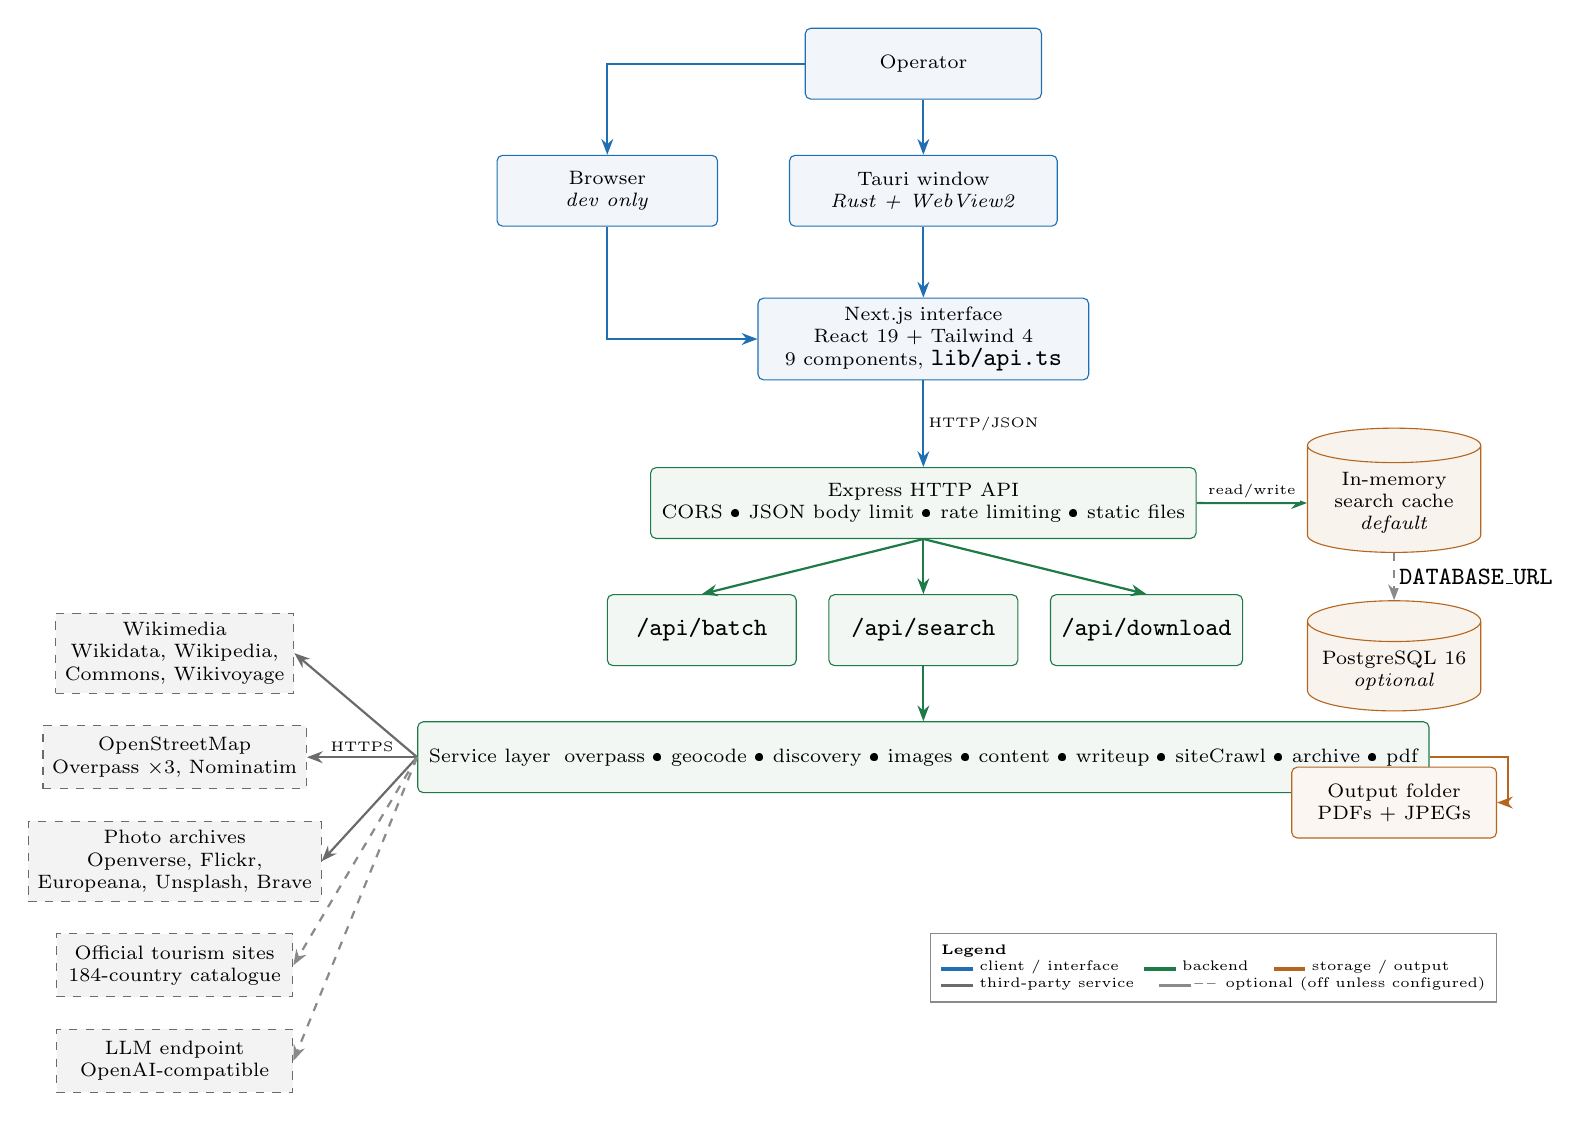
\begin{tikzpicture}[node distance=5mm]

% ---- clients
\node[box=cFront, minimum width=30mm] (user) {Operator};
\node[box=cFront, below=7mm of user, minimum width=34mm] (win)
  {Tauri window\\\textit{Rust + WebView2}};
\node[box=cFront, left=9mm of win, minimum width=28mm] (browser)
  {Browser\\\textit{dev only}};

% ---- frontend
\node[box=cFront, below=9mm of win, minimum width=42mm] (ui)
  {Next.js interface\\React 19 + Tailwind 4\\\scriptsize 9 components,
   \code{lib/api.ts}};

% ---- backend
\node[box=cBack, below=11mm of ui, minimum width=52mm] (api)
  {Express HTTP API\\\scriptsize CORS \textbullet\ JSON body limit \textbullet\
   rate limiting \textbullet\ static files};

\node[box=cBack, below=7mm of api, minimum width=24mm] (rsearch) {\code{/api/search}};
\node[box=cBack, right=4mm of rsearch, minimum width=24mm] (rdl) {\code{/api/download}};
\node[box=cBack, left=4mm of rsearch, minimum width=24mm] (rbatch) {\code{/api/batch}};

\node[box=cBack, below=7mm of rsearch, minimum width=74mm] (svc)
  {Service layer \;\scriptsize overpass \textbullet\ geocode \textbullet\ discovery
   \textbullet\ images \textbullet\ content \textbullet\ writeup \textbullet\
   siteCrawl \textbullet\ archive \textbullet\ pdf};

% ---- storage
\node[db, right=14mm of api, minimum width=22mm] (mem) {In-memory\\search cache\\\textit{default}};
\node[db, below=6mm of mem, minimum width=22mm] (pg) {PostgreSQL 16\\\textit{optional}};
\node[box=cData, below=7mm of pg, minimum width=26mm] (disk)
  {Output folder\\\scriptsize PDFs + JPEGs};

% ---- external
\node[ext, left=14mm of svc, minimum width=30mm] (osm)
  {OpenStreetMap\\\scriptsize Overpass $\times$3, Nominatim};
\node[ext, above=4mm of osm, minimum width=30mm] (wiki)
  {Wikimedia\\\scriptsize Wikidata, Wikipedia,\\Commons, Wikivoyage};
\node[ext, below=4mm of osm, minimum width=30mm] (photo)
  {Photo archives\\\scriptsize Openverse, Flickr,\\Europeana, Unsplash, Brave};
\node[ext, below=4mm of photo, minimum width=30mm] (tour)
  {Official tourism sites\\\scriptsize 184-country catalogue};
\node[ext, below=4mm of tour, minimum width=30mm] (llm)
  {LLM endpoint\\\scriptsize OpenAI-compatible};

% ---- flows
\draw[fl=cFront] (user) -- (win);
\draw[fl=cFront] (user.west) -| (browser);
\draw[fl=cFront] (win) -- (ui);
\draw[fl=cFront] (browser) |- (ui.west);
\draw[fl=cFront] (ui) -- node[lbl,right]{HTTP/JSON} (api);
\draw[fl=cBack] (api) -- (rsearch);
\draw[fl=cBack] (api.south) -- (rbatch.north);
\draw[fl=cBack] (api.south) -- (rdl.north);
\draw[fl=cBack] (rsearch) -- (svc);
\draw[fl=cBack] (api) -- node[lbl,above]{read/write} (mem);
\draw[flo] (mem) -- node[lbl,right]{\code{DATABASE\_URL}} (pg);
\draw[fl=cData] (svc.east) -- ++(10mm,0) |- (disk);
\draw[fl=cExt] (svc.west) -- node[lbl,above]{HTTPS} (osm.east);
\draw[fl=cExt] (svc.west) -- (wiki.east);
\draw[fl=cExt] (svc.west) -- (photo.east);
\draw[flo] (svc.west) -- (tour.east);
\draw[flo] (svc.west) -- (llm.east);

% ---- legend
\node[draw=cNote, fill=white, align=left, font=\tiny, below=8mm of disk,
      anchor=north east, inner sep=4pt] (leg) at ($(disk.south east)+(0,-4mm)$) {%
  \textbf{Legend}\\
  \textcolor{cFront}{\rule{4mm}{1.4pt}} client / interface \quad
  \textcolor{cBack}{\rule{4mm}{1.4pt}} backend \quad
  \textcolor{cData}{\rule{4mm}{1.4pt}} storage / output\\
  \textcolor{cExt}{\rule{4mm}{1.4pt}} third-party service \quad
  \textcolor{cNote}{\rule{4mm}{1.4pt}}\,--\,--\, optional (off unless configured)
};
\end{tikzpicture}}
\caption[System architecture]{System architecture. Solid arrows are paths every
run takes; dashed arrows are optional and inactive unless the corresponding
setting or API key is supplied. The PostgreSQL store, the LLM endpoint, the
keyed photo archives and the tourism-site crawl are all optional.}
\label{fig:arch}
\end{figure}

\paragraph{Reading the diagram.} Three observations matter more than the boxes
themselves.

\begin{itemize}
\item \textbf{One backend, three front doors.} The browser, the packaged
executable and the Tauri window all speak to the same Express API over HTTP. The
desktop shell does not reimplement anything; it launches the same server binary
as a child process and points a WebView at it.
\item \textbf{Storage is incidental.} The only persistent artefact the
application is trying to produce is the output folder. The caches exist so that
an export can refer back to the search that produced it.
\item \textbf{Most of the work is outbound.} The service layer's job is
orchestrating roughly a dozen third-party APIs. This is why availability of those
services, not local compute, dominates runtime behaviour.
\end{itemize}

% =====================================================================
\chapter{Application Flow}
\label{sec:flow}

\section{Search request lifecycle}

Figure~\ref{fig:search} traces one search from the operator pressing
\emph{Search} to results appearing. The stage names are the literal values the
backend reports through its progress channel, read from
\file{backend/src/services/search.ts}.

\begin{figure}[H]
\centering
\resizebox{!}{0.78\textheight}{%
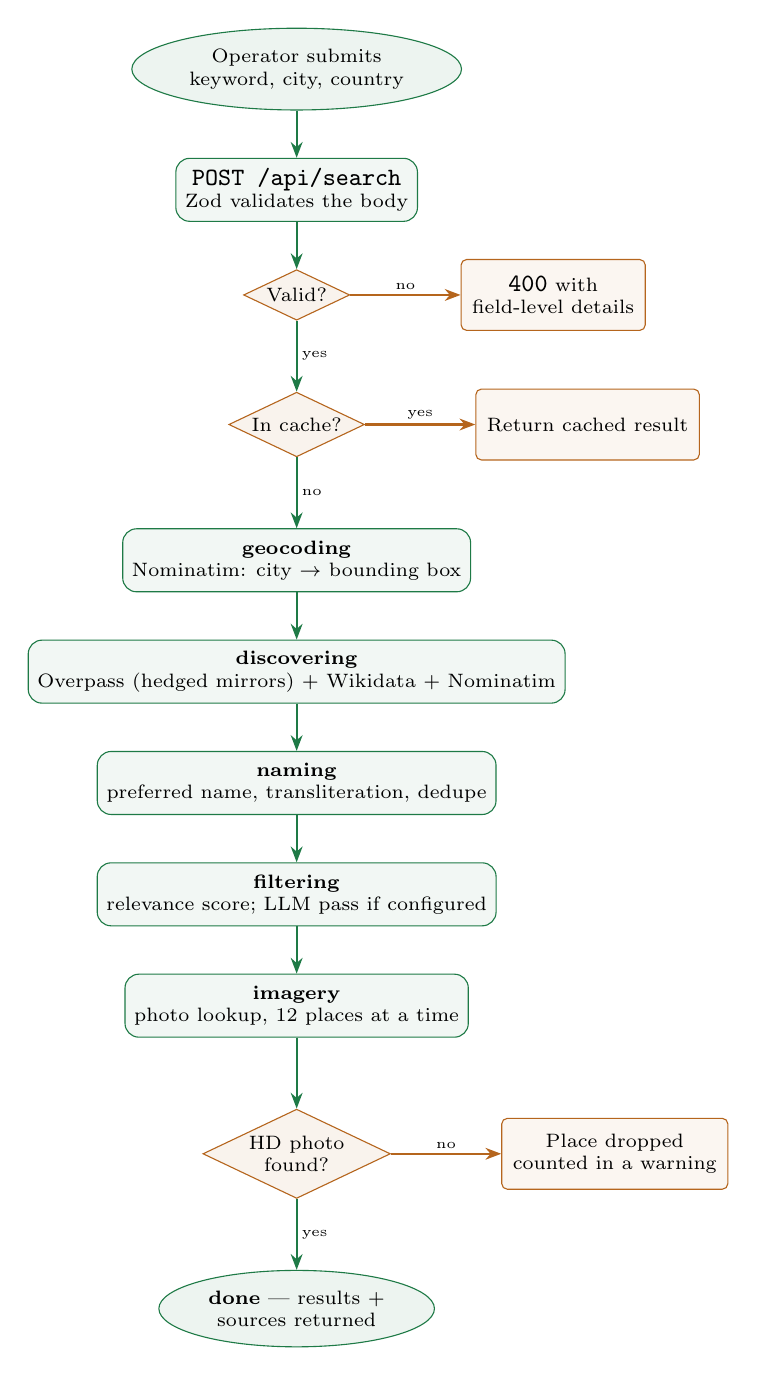
\begin{tikzpicture}[node distance=6mm]
\node[term] (start) {Operator submits\\keyword, city, country};
\node[proc, below=of start] (post) {\code{POST /api/search}\\\scriptsize Zod validates the body};
\node[dec, below=of post] (valid) {Valid?};
\node[box=cData, right=14mm of valid] (e400) {\code{400} with\\field-level details};
\node[dec, below=9mm of valid] (cached) {In cache?};
\node[box=cData, right=14mm of cached] (hit) {Return cached result};
\node[proc, below=9mm of cached] (geo) {\textbf{geocoding}\\\scriptsize Nominatim: city $\rightarrow$ bounding box};
\node[proc, below=of geo] (disc) {\textbf{discovering}\\\scriptsize Overpass (hedged mirrors) + Wikidata + Nominatim};
\node[proc, below=of disc] (name) {\textbf{naming}\\\scriptsize preferred name, transliteration, dedupe};
\node[proc, below=of name] (filt) {\textbf{filtering}\\\scriptsize relevance score; LLM pass if configured};
\node[proc, below=of filt] (img) {\textbf{imagery}\\\scriptsize photo lookup, 12 places at a time};
\node[dec, below=9mm of img] (hd) {HD photo\\found?};
\node[box=cData, right=14mm of hd] (drop) {Place dropped\\\scriptsize counted in a warning};
\node[term, below=9mm of hd] (done) {\textbf{done} --- results +\\sources returned};

\draw[fl=cBack] (start) -- (post);
\draw[fl=cBack] (post) -- (valid);
\draw[fl=cData] (valid) -- node[lbl,above]{no} (e400);
\draw[fl=cBack] (valid) -- node[lbl,right]{yes} (cached);
\draw[fl=cData] (cached) -- node[lbl,above]{yes} (hit);
\draw[fl=cBack] (cached) -- node[lbl,right]{no} (geo);
\draw[fl=cBack] (geo) -- (disc);
\draw[fl=cBack] (disc) -- (name);
\draw[fl=cBack] (name) -- (filt);
\draw[fl=cBack] (filt) -- (img);
\draw[fl=cBack] (img) -- (hd);
\draw[fl=cData] (hd) -- node[lbl,above]{no} (drop);
\draw[fl=cBack] (hd) -- node[lbl,right]{yes} (done);
\end{tikzpicture}}
\caption[Search request lifecycle]{Search request lifecycle. Bold words are the
progress stages the backend actually emits. The ``HD photo found?'' branch is
active because \code{REQUIRE\_IMAGES} defaults to true: a place with no
photograph of at least \code{MIN\_IMAGE\_WIDTH} pixels is removed from the
result rather than returned as text.}
\label{fig:search}
\end{figure}

\paragraph{Note on authentication.} No step in this flow checks an identity or a
permission, because none exists in the codebase (Section~\ref{sec:auth}). A
generic flowchart would place an authentication gate after validation; this one
does not, because that gate is not implemented.

\section{Export pipeline}

Export is a separate request. Figure~\ref{fig:export} shows it, including the
two decisions that most affect what the operator ends up with.

\begin{figure}[H]
\centering
\resizebox{!}{0.78\textheight}{%
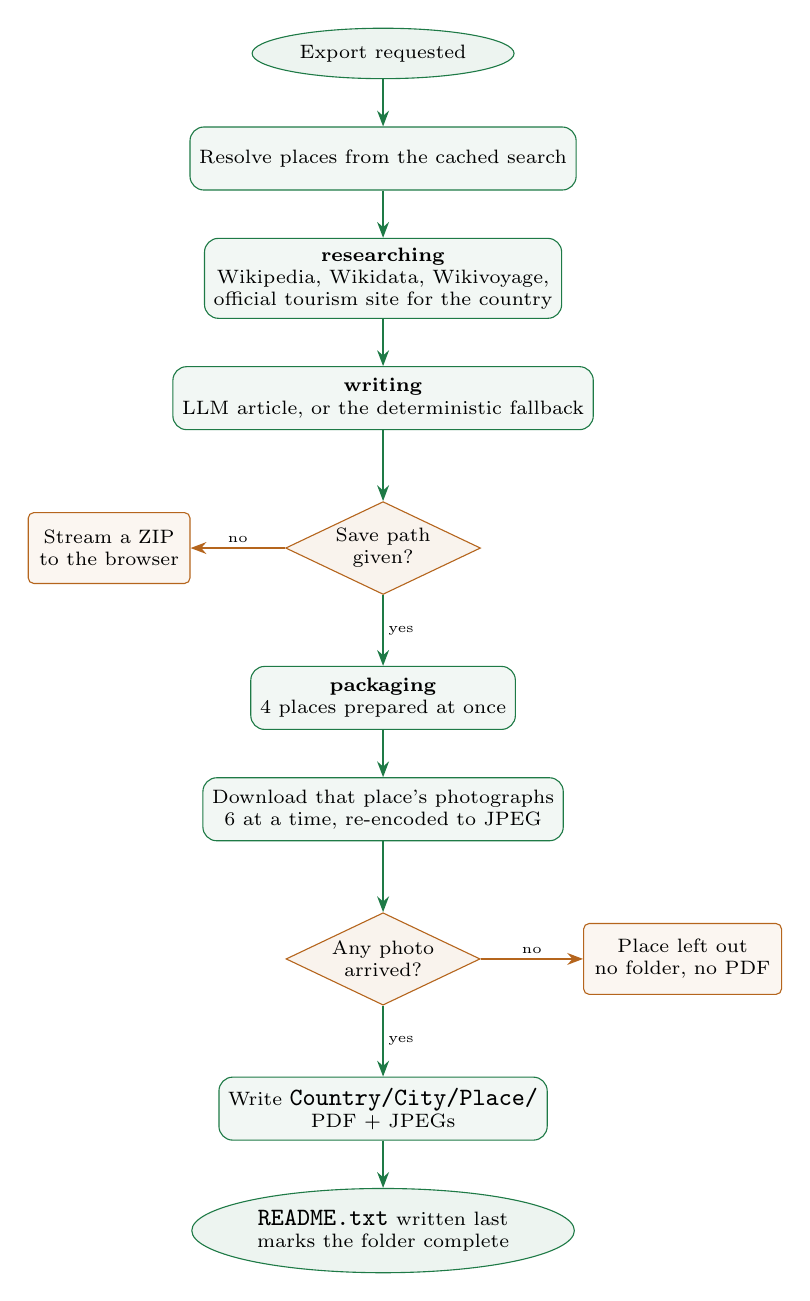
\begin{tikzpicture}[node distance=6mm]
\node[term] (s) {Export requested};
\node[proc, below=of s] (res) {Resolve places from the cached search};
\node[proc, below=of res] (crawl) {\textbf{researching}\\\scriptsize Wikipedia, Wikidata, Wikivoyage,\\official tourism site for the country};
\node[proc, below=of crawl] (wr) {\textbf{writing}\\\scriptsize LLM article, or the deterministic fallback};
\node[dec, below=9mm of wr] (path) {Save path\\given?};
\node[box=cData, left=12mm of path] (zip) {Stream a ZIP\\to the browser};
\node[proc, below=9mm of path] (pipe) {\textbf{packaging}\\\scriptsize 4 places prepared at once};
\node[proc, below=of pipe] (dl) {Download that place's photographs\\\scriptsize 6 at a time, re-encoded to JPEG};
\node[dec, below=9mm of dl] (got) {Any photo\\arrived?};
\node[box=cData, right=13mm of got] (skip) {Place left out\\\scriptsize no folder, no PDF};
\node[proc, below=9mm of got] (write) {Write \code{Country/City/Place/}\\\scriptsize PDF + JPEGs};
\node[term, below=of write] (fin) {\code{README.txt} written last\\\scriptsize marks the folder complete};

\draw[fl=cBack] (s) -- (res);
\draw[fl=cBack] (res) -- (crawl);
\draw[fl=cBack] (crawl) -- (wr);
\draw[fl=cBack] (wr) -- (path);
\draw[fl=cData] (path) -- node[lbl,above]{no} (zip);
\draw[fl=cBack] (path) -- node[lbl,right]{yes} (pipe);
\draw[fl=cBack] (pipe) -- (dl);
\draw[fl=cBack] (dl) -- (got);
\draw[fl=cData] (got) -- node[lbl,above]{no} (skip);
\draw[fl=cBack] (got) -- node[lbl,right]{yes} (write);
\draw[fl=cBack] (write) -- (fin);
\end{tikzpicture}}
\caption[Export pipeline]{Export pipeline. A named folder receives the files
directly; only a browser download produces a ZIP, because a browser cannot
download a directory. A place whose photographs all fail to download is left out
entirely rather than exported as a write-up with an empty folder.}
\label{fig:export}
\end{figure}

% =====================================================================
\chapter{Frontend Technology}
\label{sec:frontend}

\section{Framework and rendering}

The interface is a \textbf{Next.js 15.5.22} application using the App Router,
built on \textbf{React 19.2.8}. It has exactly one route: \file{frontend/app/page.tsx},
with \file{app/layout.tsx} supplying the document shell.

Rendering differs between development and the shipped product, and this is
deliberate --- \file{frontend/next.config.mjs} switches on an environment variable:

\begin{itemize}
\item \textbf{Development}: the normal Next.js dev server on port 3000, with hot
reload, calling the backend on port 4000.
\item \textbf{Packaged}: \code{build-exe.mjs} sets \code{NEXT\_EXPORT=1}, which
turns on \code{output: 'export'}. Next emits a fully static bundle with no Node
server of its own, and the Express backend serves those files from
\code{config.webDir}. Image optimisation is disabled in this mode because there
is no optimisation server in the packaged binary.
\end{itemize}

This is why the packaged product is a single executable rather than two
processes: the interface becomes static files that the API server hosts.

\section{Components and state}

Nine components live in \file{frontend/components/}:

\begin{longtable}{@{}>{\raggedright\arraybackslash}p{4.1cm}>{\raggedright\arraybackslash}p{10.6cm}@{}}
\caption{Interface components and their responsibilities}\label{tab:components}\\
\toprule
\textbf{Component} & \textbf{Responsibility}\\
\midrule
\endfirsthead
\toprule
\textbf{Component} & \textbf{Responsibility}\\
\midrule
\endhead
\bottomrule
\endfoot
\file{PlaceFinder.tsx}   & Top-level container; owns the search result and switches between single and batch modes\\
\file{HeroSearch.tsx}    & Landing state and the explanation of what the export contains\\
\file{SearchForm.tsx}    & Keyword, city and country inputs, category chips, output folder picker, source list, extra source links\\
\file{ResultsPanel.tsx}  & Result list, sorting, export controls, data-source disclosure\\
\file{PlaceCard.tsx}     & One place: photographs, summary, outbound links\\
\file{MapView.tsx}       & Map of the result area\\
\file{BatchPanel.tsx}    & CSV upload, batch job control, per-region progress and retry\\
\file{SearchProgress.tsx}& Live progress for a running search\\
\file{BuildStamp.tsx}    & Shows the build and commit the server reports\\
\end{longtable}

\paragraph{State management.} There is \textbf{no state management library}. The
\file{frontend/package.json} dependency list contains only \code{next},
\code{react} and \code{react-dom}; there is no Redux, Zustand, Jotai, Recoil,
React Query or SWR. State is held in React hooks --- 51 \code{useState}, 18
\code{useEffect}, 13 \code{useCallback}, 10 \code{useRef} and 7 \code{useMemo}
across the component tree --- and passed down by props. For an application with
one screen and one long-running operation, this avoids a dependency without
obvious cost.

\section{Styling}

\textbf{Tailwind CSS 4.3.3}, wired through \code{@tailwindcss/postcss} in
\file{frontend/postcss.config.mjs}. Tailwind~4 is configured in CSS rather than
JavaScript: \file{app/globals.css} begins with \code{@import 'tailwindcss'} and
declares the theme there. \textbf{There is no \file{tailwind.config.js}}, which
is expected for this version and is not a missing file.

All styling is utility classes in the components plus that one stylesheet. No
CSS-in-JS library, CSS modules or component library is present.

\section{Map rendering}

\file{MapView.tsx} embeds an \code{<iframe>} pointing at
\url{https://www.openstreetmap.org/export/embed.html} with a bounding box derived
from the result set. \textbf{No mapping library is used} --- there is no Leaflet,
Mapbox GL or Google Maps JavaScript SDK in the dependency tree. This keeps the
bundle small and needs no API key, at the cost of interactive map features.

\section{Communication with the backend}

All network access goes through \file{frontend/lib/api.ts} using the browser
\code{fetch} API. The base URL is \code{process.env.NEXT\_PUBLIC\_API\_BASE\_URL},
defaulting to \code{http://localhost:4000}. \file{frontend/lib/types.ts} mirrors
the backend response shapes.

Long operations are followed by \textbf{polling}, not pushed: a search returns a
progress identifier and the interface polls \file{/api/search/progress/:id};
batch jobs poll \file{/api/batch/:jobId}. No WebSocket or server-sent-events
transport is present.

\section{Accessibility and responsive design}

Responsive behaviour comes from Tailwind's breakpoint utilities. \textbf{No
accessibility tooling is configured} --- there is no \code{eslint-plugin-jsx-a11y},
axe integration or automated accessibility test in the repository. This is
recorded as an absence, not a defect: it means accessibility is unverified rather
than known to be poor.

% =====================================================================
\chapter{Backend Technology}
\label{sec:backend}

\section{Runtime and framework}

\textbf{Node.js} running \textbf{Express 4.22.2}. \file{backend/package.json}
declares \code{engines.node >= 20}; the machine this document was produced on runs
\ver{v24.18.0}. The package is an ES module (\code{"type": "module"}) written
entirely in TypeScript and executed through \code{tsx} in development.

\section{Entry point and middleware}

\file{backend/src/index.ts} assembles the application in this order:

\begin{enumerate}
\item \textbf{CORS} (\code{cors} 2.8.6) restricted to the configured origins.
\item \textbf{JSON body parsing} capped at \code{maxRequestBodyBytes} (8\,MB) ---
the limit exists because batch requests carry an uploaded CSV.
\item \textbf{Health endpoint} \code{GET /api/health}, which also probes
connectivity so the application notices the network returning.
\item \textbf{Three routers} mounted under \code{/api}.
\item \textbf{Static files} from \code{config.webDir} --- present only in the
packaged build, where this serves the exported interface.
\item \textbf{404 handler}, then a final \textbf{error handler}.
\end{enumerate}

On startup the server also selects a port: it tries \code{PORT} (default 4000)
and walks upward if the port is occupied, and if an instance is already running
it opens that one instead of starting a second.

\section{Service layer}

Routes are thin; the work lives in \file{backend/src/services/}. The significant
modules:

\begin{longtable}{@{}>{\raggedright\arraybackslash}p{3.5cm}>{\raggedright\arraybackslash}p{11.2cm}@{}}
\caption{Backend service modules}\label{tab:services}\\
\toprule
\textbf{Module} & \textbf{Responsibility}\\
\midrule
\endfirsthead
\toprule
\textbf{Module} & \textbf{Responsibility}\\
\midrule
\endhead
\bottomrule
\endfoot
\file{search.ts}      & Orchestrates a search: geocode, discover, name, filter, illustrate\\
\file{overpass.ts}    & Overpass queries; mirror racing, health memory, selector merging\\
\file{geocode.ts}     & Nominatim lookups, city to bounding box and area id\\
\file{discovery.ts}   & Extra places from Wikidata and Nominatim beyond Overpass\\
\file{images.ts}      & Photo lookup across archives, HD filtering, Commons gateway fallback\\
\file{imageSources.ts}& Flickr, Europeana, Brave and Commons geo-search clients\\
\file{content.ts}     & Wikipedia, Wikidata and Wikivoyage extracts per place\\
\file{siteCrawl.ts}   & Shallow, robots-respecting crawl of a country's official tourism site\\
\file{extraSources.ts}& Reduces fetched pages to text and mines passages about a place\\
\file{writeup.ts}     & LLM article generation plus a deterministic fallback\\
\file{llm.ts}         & OpenAI-compatible chat client; Ollama auto-detection\\
\file{translate.ts}   & Name translation and transliteration via the LLM\\
\file{embeddings.ts}  & Optional embeddings for semantic de-duplication\\
\file{semanticDedupe.ts}& Collapses places that are the same thing under two names\\
\file{archive.ts}     & Builds the output, to a folder or a ZIP, and renders each PDF\\
\file{pdf.ts}         & PDFKit document construction\\
\file{batch.ts}       & Multi-city job runner with resume, retry and cancellation\\
\file{cache.ts}       & Search store: in-memory, or PostgreSQL when configured\\
\file{progress.ts}    & Stage reporting consumed by the interface\\
\end{longtable}

\section{Cross-cutting libraries}

\file{backend/src/lib/} holds the infrastructure the services share:
\file{http.ts} (one fetch wrapper with per-host rate limiting, retries, timeouts
and cancellation), \file{cancel.ts} (ambient \code{AbortSignal} propagation),
\file{concurrency.ts} (bounded parallel helpers), \file{robots.ts} (robots.txt
parsing), \file{publicUrl.ts} (SSRF protection for images from untrusted
origins), \file{rateLimit.ts}, \file{sanitize.ts} (safe path segments),
\file{csv.ts}, \file{taxonomy.ts} (keyword to OpenStreetMap tag mapping),
\file{connectivity.ts} (offline detection) and \file{factCheck.ts}.

\section{Background work}

Batch processing is the only long-running work. \file{services/batch.ts} runs one
job at a time in the same process, writing state to disk so an interrupted job
can resume. There is \textbf{no job queue, scheduler or worker process} --- no
cron, BullMQ, Agenda or similar appears in the dependency tree.

% =====================================================================
\chapter{Programming Languages}
\label{sec:languages}

\begin{longtable}{@{}>{\raggedright\arraybackslash}p{2.6cm}>{\raggedright\arraybackslash}p{3.4cm}>{\raggedright\arraybackslash}p{4.6cm}>{\raggedright\arraybackslash}p{4.4cm}@{}}
\caption{Languages present in the repository}\label{tab:languages}\\
\toprule
\textbf{Language} & \textbf{Where} & \textbf{Responsibility} & \textbf{Evidence}\\
\midrule
\endfirsthead
\toprule
\textbf{Language} & \textbf{Where} & \textbf{Responsibility} & \textbf{Evidence}\\
\midrule
\endhead
\bottomrule
\endfoot
TypeScript & \file{backend/src}, \file{frontend} & All application code, both halves &
\file{.ts}/\file{.tsx}; \file{tsconfig.json} in each package\\
JavaScript (ESM) & Build scripts, test files, config &
Packaging, Next and PostCSS config, tests &
\file{build-exe.mjs}, \file{build-desktop.mjs}, \file{*.test.mjs}, \file{next.config.mjs}\\
Rust & \file{desktop/src-tauri/src} & Desktop shell: window, child process supervision, job objects &
\file{main.rs}; \file{Cargo.toml} \code{edition 2021}, \code{rust-version 1.77.2}\\
CSS & \file{frontend/app/globals.css} & Theme tokens and Tailwind import & \file{globals.css}\\
SQL & \file{backend/src/services/cache.ts} & Table creation and queries for the optional store &
SQL literals inside \file{cache.ts}\\
JSON & Throughout & Manifests, lockfiles, Tauri configuration & \file{package.json}, \file{tauri.conf.json}\\
YAML & \file{docker-compose.yml} & PostgreSQL service definition & \file{docker-compose.yml}\\
PowerShell & \file{backend/src/routes/batch.ts} & Native folder-picker dialog on Windows &
\code{execFile('powershell.exe', \ldots)} in \file{batch.ts}\\
\end{longtable}

\paragraph{Not present.} No Python, Java, Go, PHP, Ruby or C\# source appears in
the repository. \code{sharp} contains native binaries, but the project itself
contributes no compiled C/C++ source.

% =====================================================================
\chapter{Frameworks}
\label{sec:frameworks}

\begin{description}[style=unboxed,leftmargin=0pt]
\item[Express 4.22.2 --- backend HTTP layer.] Supplies routing, middleware
composition, body parsing, static file serving and centralised error handling.
Used through three \code{Router} instances mounted under \code{/api}. Related
files: \file{backend/src/index.ts}, \file{backend/src/routes/}. Note this is the
Express~4 line, not Express~5.

\item[Next.js 15.5.22 --- frontend framework.] Supplies the App Router, the
development server, the production bundler and the static export used by the
packaged build. Configured in \file{frontend/next.config.mjs}, which also
declares the remote image hosts the interface is permitted to load photographs
from.

\item[React 19.2.8 --- UI library.] The component and hook model the entire
interface is written against. Strict mode is enabled
(\code{reactStrictMode: true}).

\item[Tauri 2 --- desktop shell framework.] A Rust framework that renders a web
application in the operating system's own WebView. Here it does three things:
opens the window, starts the packaged server as a child process, and ties that
child's lifetime to its own using a Windows job object so the server cannot
outlive the window. Configured in \file{desktop/src-tauri/tauri.conf.json}.

\item[Tailwind CSS 4.3.3 --- styling framework.] Utility classes plus a
CSS-declared theme. Operates entirely at build time through PostCSS.
\end{description}

\paragraph{Testing framework.} There is none, deliberately. Tests run on
\code{node:test}, the runner built into Node, invoked as
\code{node --import tsx --test}. See Section~\ref{sec:testing}.

% =====================================================================
\chapter{Libraries and Important Dependencies}
\label{sec:libs}

The project declares a small dependency surface: \textbf{8 runtime dependencies}
and \textbf{11 development dependencies} in the backend, and \textbf{3 runtime
dependencies} in the frontend. Versions below are the \emph{locked} versions from
\file{package-lock.json} (lockfile version 3), which is what actually installs.

\begin{longtable}{@{}>{\raggedright\arraybackslash}p{2.9cm}>{\raggedright\arraybackslash}p{1.6cm}>{\raggedright\arraybackslash}p{2.0cm}>{\raggedright\arraybackslash}p{7.6cm}@{}}
\caption{Backend runtime dependencies (direct)}\label{tab:deps-backend}\\
\toprule
\textbf{Package} & \textbf{Declared} & \textbf{Locked} & \textbf{Why the project needs it}\\
\midrule
\endfirsthead
\toprule
\textbf{Package} & \textbf{Declared} & \textbf{Locked} & \textbf{Why the project needs it}\\
\midrule
\endhead
\bottomrule
\endfoot
\code{express}  & \code{\^{}4.21.2} & \ver{4.22.2} & HTTP server, routing and middleware. Required for startup\\
\code{cors}     & \code{\^{}2.8.5}  & \ver{2.8.6}  & Lets the dev interface on port 3000 call the API on port 4000\\
\code{dotenv}   & \code{\^{}16.4.7} & \ver{16.6.1} & Loads the \file{.env} that sits beside the packaged executable\\
\code{zod}      & \code{\^{}3.24.1} & \ver{3.25.76}& Validates every request body and query string before it reaches a service\\
\code{pdfkit}   & \code{\^{}0.15.2} & \ver{0.15.2} & Generates the per-place PDF and the search summary\\
\code{sharp}    & \code{\^{}0.33.5} & \ver{0.33.5} & Converts and re-encodes every downloaded photograph. Native binary\\
\code{archiver} & \code{\^{}7.0.1}  & \ver{7.0.1}  & Streams the ZIP used for browser downloads\\
\code{pg}       & \code{\^{}8.13.1} & \ver{8.22.0} & PostgreSQL client. Loaded lazily and only when \code{DATABASE\_URL} is set\\
\end{longtable}

\begin{longtable}{@{}>{\raggedright\arraybackslash}p{3.3cm}>{\raggedright\arraybackslash}p{1.6cm}>{\raggedright\arraybackslash}p{2.0cm}>{\raggedright\arraybackslash}p{7.2cm}@{}}
\caption{Development and build dependencies}\label{tab:deps-dev}\\
\toprule
\textbf{Package} & \textbf{Declared} & \textbf{Locked} & \textbf{Role}\\
\midrule
\endfirsthead
\toprule
\textbf{Package} & \textbf{Declared} & \textbf{Locked} & \textbf{Role}\\
\midrule
\endhead
\bottomrule
\endfoot
\code{typescript}    & \code{\^{}5.7.3}  & \ver{5.9.3}  & Type checking and compilation (both packages)\\
\code{tsx}           & \code{\^{}4.19.2} & \ver{4.23.5} & Runs TypeScript directly in development and for tests\\
\code{esbuild}       & \code{\^{}0.28.1} & \ver{0.28.1} & Bundles the server into one file before packaging\\
\code{@yao-pkg/pkg}  & \code{\^{}6.22.0} & \ver{6.22.0} & Produces the single-file Windows executable\\
\code{@types/*}      & various           & ---          & Type definitions for node, express, cors, pg, pdfkit, archiver, react\\
\end{longtable}

\begin{longtable}{@{}>{\raggedright\arraybackslash}p{3.5cm}>{\raggedright\arraybackslash}p{1.8cm}>{\raggedright\arraybackslash}p{2.0cm}>{\raggedright\arraybackslash}p{7.0cm}@{}}
\caption{Frontend dependencies}\label{tab:deps-frontend}\\
\toprule
\textbf{Package} & \textbf{Declared} & \textbf{Locked} & \textbf{Role}\\
\midrule
\endfirsthead
\toprule
\textbf{Package} & \textbf{Declared} & \textbf{Locked} & \textbf{Role}\\
\midrule
\endhead
\bottomrule
\endfoot
\code{next}                  & \code{\^{}15.1.6} & \ver{15.5.22} & Framework, dev server, bundler, static export\\
\code{react}                 & \code{\^{}19.0.0} & \ver{19.2.8}  & UI library\\
\code{react-dom}             & \code{\^{}19.0.0} & \ver{19.2.8}  & DOM renderer\\
\code{tailwindcss}           & \code{\^{}4.0.0}  & \ver{4.3.3}   & Styling (dev dependency; compiled away at build)\\
\code{@tailwindcss/postcss}  & \code{\^{}4.0.0}  & \ver{4.3.3}   & PostCSS plugin that runs Tailwind\\
\end{longtable}

\paragraph{Transitive dependencies.} Not enumerated here. The direct surface
above is what the project imports; \code{sharp} and \code{next} bring the largest
transitive trees, and \code{sharp} additionally ships platform-specific native
binaries, which is why \file{build-exe.mjs} copies it and its dependency closure
next to the executable rather than relying on the bundler.

\paragraph{Notably absent.} No HTTP client library (the built-in \code{fetch} is
used), no logging framework (\code{console} with bracketed prefixes), no ORM, no
authentication library, no test framework, no state management library and no UI
component library.

% =====================================================================
\chapter{UI Libraries and Styling}
\label{sec:ui}

This chapter exists to record an absence precisely, because ``which component
library?'' is usually the first question asked of a frontend.

\begin{longtable}{@{}>{\raggedright\arraybackslash}p{3.8cm}>{\raggedright\arraybackslash}p{4.0cm}>{\raggedright\arraybackslash}p{6.8cm}@{}}
\caption{UI technology: what is present and what is not}\label{tab:ui}\\
\toprule
\textbf{Category} & \textbf{In this project} & \textbf{Evidence}\\
\midrule
\endfirsthead
\toprule
\textbf{Category} & \textbf{In this project} & \textbf{Evidence}\\
\midrule
\endhead
\bottomrule
\endfoot
CSS framework        & Tailwind CSS 4.3.3 & \file{postcss.config.mjs}, \file{app/globals.css}\\
Component library    & \textbf{None} & No MUI, Chakra, Ant Design, shadcn/ui or Radix in \file{package.json}\\
Icon library         & \textbf{None} & No icon package; inline SVG and text are used\\
Charting library     & \textbf{None} & No Chart.js, Recharts or D3\\
Animation library    & \textbf{None} & No Framer Motion; transitions are CSS utilities\\
Design system        & \textbf{None formalised} & Colour tokens declared in \file{globals.css}\\
Mapping library      & \textbf{None} & OpenStreetMap \code{<iframe>} in \file{MapView.tsx}\\
Font loading         & Default stack & No \code{next/font} usage or webfont import found\\
\end{longtable}

Every control in the interface --- buttons, chips, the folder picker, the progress
bars, the collapsible source list --- is a hand-written React component styled
with Tailwind utilities. The practical consequence is a very small dependency
surface and no component-library upgrade burden, in exchange for all accessibility
and interaction behaviour being the project's own responsibility.

% =====================================================================
\chapter{Database and Data Layer}
\label{sec:data}

\section{What the data layer actually is}

\textbf{This application has no application database in the usual sense.} It
stores no users, no documents and no domain records. What it has is a
\emph{search cache} with two interchangeable implementations, selected at
startup in \file{backend/src/services/cache.ts}:

\begin{itemize}
\item \textbf{In-memory store (default).} A \code{MemoryStore} class holding
recent search results in process memory. Lost on restart. This is what runs
unless the operator configures otherwise.
\item \textbf{PostgreSQL store (opt-in).} A \code{PostgresStore} used only when
\code{DATABASE\_URL} is set. The \code{pg} driver is imported dynamically so the
dependency is never loaded otherwise.
\end{itemize}

The selection is not merely conditional, it is \emph{forgiving}: if
\code{DATABASE\_URL} is set but the database cannot be reached, the application
logs the failure and falls back to the in-memory store rather than refusing to
start. This is visible in \file{cache.ts} and matters operationally --- a
database outage degrades the cache, it does not take the product down.

\begin{figure}[H]
\centering
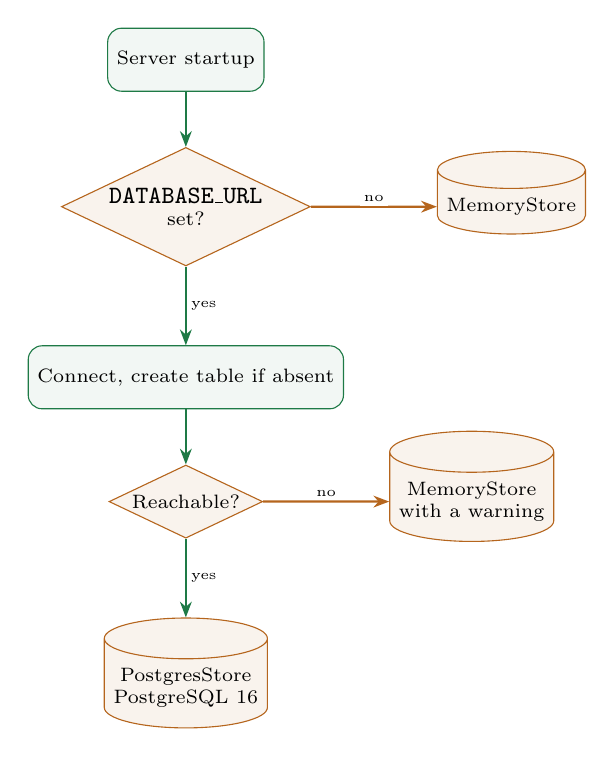
\begin{tikzpicture}[node distance=7mm]
\node[proc] (start) {Server startup};
\node[dec, below=of start] (set) {\code{DATABASE\_URL}\\set?};
\node[db, right=16mm of set] (mem1) {MemoryStore};
\node[proc, below=10mm of set] (try) {Connect, create table if absent};
\node[dec, below=of try] (ok) {Reachable?};
\node[db, below=10mm of ok] (pg) {PostgresStore\\\scriptsize PostgreSQL 16};
\node[db, right=16mm of ok] (mem2) {MemoryStore\\\scriptsize with a warning};

\draw[fl=cBack] (start) -- (set);
\draw[fl=cData] (set) -- node[lbl,above]{no} (mem1);
\draw[fl=cBack] (set) -- node[lbl,right]{yes} (try);
\draw[fl=cBack] (try) -- (ok);
\draw[fl=cBack] (ok) -- node[lbl,right]{yes} (pg);
\draw[fl=cData] (ok) -- node[lbl,above]{no} (mem2);
\end{tikzpicture}
\caption[Storage selection]{How the search store is chosen at startup. The
fallback path on the right is why the application starts successfully with no
database present, which is the default configuration.}
\label{fig:storage}
\end{figure}

\section{Schema}

The schema is created by the application itself when the PostgreSQL store
initialises --- there is \textbf{no migration tool and no migration directory}.
No Prisma, Drizzle, TypeORM, Sequelize or Knex appears anywhere; SQL is written
as string literals and executed through \code{pg}. There are no entities,
relationships or constraints beyond the single cache table, so an
entity-relationship diagram would show one box and no relationships; it is
omitted as uninformative rather than fabricated.

\section{Real persistence: the filesystem}

The output the operator cares about is written to disk as a directory tree:

\begin{verbatim}
<chosen folder>/
    <Country>/
        <City>/
            <Place name>/
                <Place name>_details.pdf
                <Place name>_01.jpeg  ...
            README.txt
\end{verbatim}

\code{README.txt} is written last, which makes it a completion marker: a batch
resume treats a region folder containing one as finished, and rebuilds one
without. Path segments are sanitised by \file{lib/sanitize.ts} before they touch
the filesystem.

\paragraph{Secrets.} No credentials appear in this document. The
\file{docker-compose.yml} in the repository contains development-only credentials
for a local container; those are not reproduced here and must not be used for any
reachable deployment.

% =====================================================================
\chapter{Authentication and Authorization}
\label{sec:auth}

\textbf{No authentication or authorization is implemented in this repository.}

This is a verified absence, not an omission from this document. The following
were searched for across \file{backend/src}, \file{frontend/app},
\file{frontend/components} and \file{frontend/lib}: \code{passport},
\code{jsonwebtoken}, JWT handling, \code{bcrypt}, \code{argon2}, session
middleware, OAuth or OIDC flows, login or signup handlers, and any
\code{authenticate} routine. Three textual matches were found and each was
inspected and ruled out:

\begin{itemize}
\item \file{services/images.ts} --- the word ``session'' inside a code comment.
\item \file{services/siteCrawl.ts} --- \code{login|signin|register|account} inside
a regular expression that \emph{excludes} such pages from being crawled.
\item \file{components/BatchPanel.tsx} --- ``session'' in a comment and a UI label.
\end{itemize}

No route carries an authentication guard; no \code{req.user},
\code{requireAuth} or \code{Bearer} token check exists in
\file{backend/src/routes/} or \file{index.ts}.

\paragraph{Outbound credentials are a different thing.} The \code{Authorization}
headers that do exist are sent \emph{by} this application \emph{to} third parties:
\code{Client-ID} for Unsplash (\file{services/images.ts}) and \code{Bearer} for
the LLM endpoint (\file{services/llm.ts}, \file{translate.ts},
\file{writeup.ts}). These authenticate the application to an external API; they
do not authenticate a user to this application. The values come from environment
variables and are not reproduced here.

\paragraph{Why this is coherent.} The product is a local desktop application
bound to \code{localhost}. The user of the program is the operator of the machine,
so there is no second party to authenticate. \textbf{The consequence must be
stated plainly: the API has no access control of any kind.} Anything that can
reach the port can search, export and read the search history. The protections
that do exist are a CORS allow-list, request-body size limits, per-route rate
limiting, and SSRF defences on image fetching --- these limit abuse, they do not
establish identity.

\paragraph{If the application were ever exposed beyond localhost} --- published to
a network interface, put behind a reverse proxy, or hosted --- authentication
would have to be added first. No authentication flowchart is provided, because
drawing one would imply an architecture that does not exist.

% =====================================================================
\chapter{API Technology}
\label{sec:api}

\section{Style and conventions}

A \textbf{REST-style JSON API over HTTP}, served by Express and mounted entirely
under \code{/api}. There is no GraphQL schema, no RPC framework, no WebSocket
server and no API versioning segment in any path. Requests and responses are
JSON, except the ZIP download, which streams binary.

Validation is uniform: every endpoint that accepts input defines a Zod schema and
rejects a bad request with HTTP \code{400} and a list of
\code{\{field, message\}} objects, so the interface can mark the offending input.

\section{Endpoints}

\begin{longtable}{@{}>{\raggedright\arraybackslash}p{1.3cm}>{\raggedright\arraybackslash}p{5.0cm}>{\raggedright\arraybackslash}p{8.4cm}@{}}
\caption{HTTP API surface (from \file{backend/src/routes/} and \file{index.ts})}\label{tab:api}\\
\toprule
\textbf{Verb} & \textbf{Path} & \textbf{Purpose}\\
\midrule
\endfirsthead
\toprule
\textbf{Verb} & \textbf{Path} & \textbf{Purpose}\\
\midrule
\endhead
\bottomrule
\endfoot
GET  & \file{/api/health}               & Status, build stamp, connectivity, engine and LLM configuration\\
POST & \code{/api/search}               & Run a search. Rate limited to 12/minute\\
GET  & \file{/api/search/progress/:id}  & Poll stage and counts for a running search\\
GET  & \code{/api/searches/:searchId}   & Retrieve a cached search result\\
GET  & \code{/api/history}              & Recent searches\\
GET  & \code{/api/sources}              & Services this install draws on; accepts \code{?country=} to name that country's official tourism site\\
GET  & \code{/api/categories}           & Category suggestions and known travel providers\\
GET  & \code{/api/google-photo}         & Photo proxy for the optional Google edition\\
POST & \code{/api/download}             & Build the export. Rate limited to 6/minute\\
POST & \code{/api/batch}                & Start a batch job from an uploaded CSV\\
POST & \code{/api/batch/preview}        & Parse a CSV and report what it contains, without running\\
GET  & \code{/api/batch/current}        & The running job, if any\\
GET  & \file{/api/batch/:jobId}         & Job state, per-region rows and notes\\
POST & \code{/api/batch/:jobId/retry}   & Re-queue failed regions\\
POST & \code{/api/batch/:jobId/cancel}  & Cancel a running job\\
POST & \code{/api/browse-folder}        & Open the native folder picker (Windows)\\
GET  & \code{/api/browse-folder}        & Poll the picker's result\\
\end{longtable}

\section{Request lifecycle}

Figure~\ref{fig:apiflow} follows one request through the layers. Note the
absence of an authentication stage --- see Section~\ref{sec:auth}.

\begin{figure}[H]
\centering
\resizebox{\textwidth}{!}{%
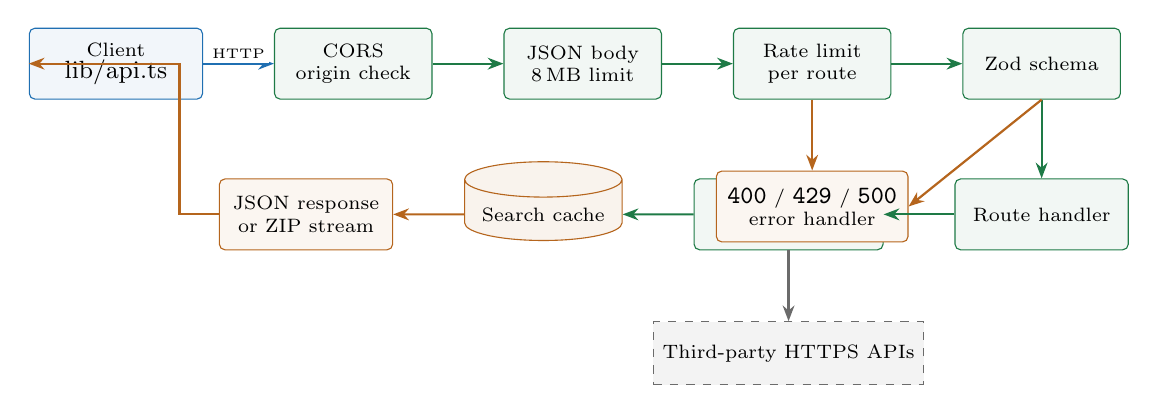
\begin{tikzpicture}[node distance=9mm]
\node[box=cFront, minimum width=22mm] (c) {Client\\\scriptsize \file{lib/api.ts}};
\node[box=cBack, right=of c, minimum width=20mm] (cors) {CORS\\\scriptsize origin check};
\node[box=cBack, right=of cors, minimum width=20mm] (body) {JSON body\\\scriptsize 8\,MB limit};
\node[box=cBack, right=of body, minimum width=20mm] (rl) {Rate limit\\\scriptsize per route};
\node[box=cBack, right=of rl, minimum width=20mm] (zod) {Zod schema};
\node[box=cBack, below=10mm of zod, minimum width=22mm] (route) {Route handler};
\node[box=cBack, left=of route, minimum width=24mm] (svc) {Service layer};
\node[db, left=of svc, minimum width=20mm] (cache) {Search cache};
\node[ext, below=9mm of svc, minimum width=30mm] (apis) {Third-party HTTPS APIs};
\node[box=cData, left=of cache, minimum width=22mm] (resp) {JSON response\\\scriptsize or ZIP stream};
\node[box=cData, below=9mm of rl, minimum width=24mm] (err) {\code{400} / \code{429} / \code{500}\\\scriptsize error handler};

\draw[fl=cFront] (c) -- node[lbl,above]{HTTP} (cors);
\draw[fl=cBack] (cors) -- (body);
\draw[fl=cBack] (body) -- (rl);
\draw[fl=cBack] (rl) -- (zod);
\draw[fl=cBack] (zod) -- (route);
\draw[fl=cBack] (route) -- (svc);
\draw[fl=cBack] (svc) -- (cache);
\draw[fl=cExt] (svc) -- (apis);
\draw[fl=cData] (cache) -- (resp);
\draw[fl=cData] (resp.west) -- ++(-5mm,0) |- (c.west);
\draw[fl=cData] (rl.south) -- (err.north);
\draw[fl=cData] (zod.south) -- (err.east);
\end{tikzpicture}}
\caption[API request lifecycle]{API request lifecycle. Every request passes CORS,
the body-size limit, the route's rate limiter and a Zod schema before a handler
sees it. There is no identity or permission stage.}
\label{fig:apiflow}
\end{figure}

\section{External APIs consumed}

Figure~\ref{fig:ext} groups the services the backend calls. Only the
OpenStreetMap and Wikimedia groups are required; everything else is optional and
inert unless configured.

\begin{figure}[H]
\centering
\resizebox{0.98\textwidth}{!}{%
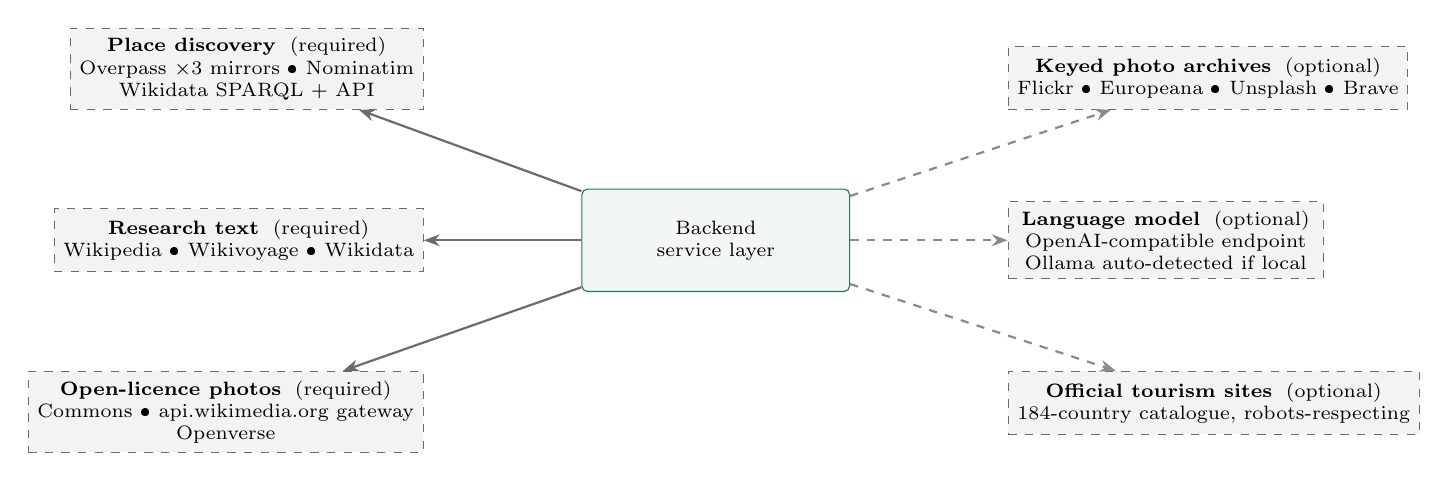
\begin{tikzpicture}[node distance=5mm]
\node[box=cBack, minimum width=34mm, minimum height=13mm] (be) {Backend\\service layer};

\node[ext, above left=10mm and 20mm of be, minimum width=40mm] (g1)
  {\textbf{Place discovery} \;\scriptsize(required)\\
   Overpass $\times$3 mirrors \textbullet\ Nominatim\\ Wikidata SPARQL + API};
\node[ext, left=20mm of be, minimum width=40mm] (g2)
  {\textbf{Research text} \;\scriptsize(required)\\
   Wikipedia \textbullet\ Wikivoyage \textbullet\ Wikidata};
\node[ext, below left=10mm and 20mm of be, minimum width=40mm] (g3)
  {\textbf{Open-licence photos} \;\scriptsize(required)\\
   Commons \textbullet\ api.wikimedia.org gateway\\ Openverse};

\node[ext, above right=10mm and 20mm of be, minimum width=40mm] (g4)
  {\textbf{Keyed photo archives} \;\scriptsize(optional)\\
   Flickr \textbullet\ Europeana \textbullet\ Unsplash \textbullet\ Brave};
\node[ext, right=20mm of be, minimum width=40mm] (g5)
  {\textbf{Language model} \;\scriptsize(optional)\\
   OpenAI-compatible endpoint\\ Ollama auto-detected if local};
\node[ext, below right=10mm and 20mm of be, minimum width=40mm] (g6)
  {\textbf{Official tourism sites} \;\scriptsize(optional)\\
   184-country catalogue, robots-respecting};

\draw[fl=cExt] (be) -- (g1);
\draw[fl=cExt] (be) -- (g2);
\draw[fl=cExt] (be) -- (g3);
\draw[flo] (be) -- (g4);
\draw[flo] (be) -- (g5);
\draw[flo] (be) -- (g6);
\end{tikzpicture}}
\caption[External service dependencies]{External services. Solid: contacted on
every search, and the application cannot produce results without them. Dashed:
skipped silently when the corresponding key or setting is absent.}
\label{fig:ext}
\end{figure}

\paragraph{API documentation.} There is \textbf{no OpenAPI/Swagger specification}
and no generated API documentation in the repository. Table~\ref{tab:api} was
compiled by reading the route files.

% =====================================================================
\chapter{Build Tools and Package Manager}
\label{sec:build}

\section{Package manager}

\textbf{npm}. Both packages carry \file{package-lock.json} at lockfile version~3;
the npm in use when this document was produced was \ver{11.16.0}. A stray
\file{pnpm-lock.yaml} exists in the \emph{parent} directory above the project
root --- Next.js warns about it when inferring its workspace root --- but the
project itself is installed with npm. There is no workspaces configuration; the
root \file{package.json} installs each package with
\code{npm --prefix <dir> install}.

\section{Compilation and bundling}

\begin{itemize}
\item \textbf{TypeScript 5.9.3} --- \code{target ES2022}, \code{strict: true} in
both packages; \code{module NodeNext} in the backend and \code{esnext} in the
frontend.
\item \textbf{tsx 4.23.5} --- runs TypeScript directly in development and under
the test runner, so there is no build step while developing the backend.
\item \textbf{esbuild 0.28.1} --- bundles the server into a single CommonJS file
in \file{pkg-stage/} before packaging.
\item \textbf{Next.js bundler} --- builds the interface; with
\code{NEXT\_EXPORT=1} it emits a static site instead of a server bundle.
\item \textbf{@yao-pkg/pkg 6.22.0} --- embeds Node plus the bundled server and the
static interface into one \code{.exe}. A maintained fork of the discontinued
\code{vercel/pkg}.
\item \textbf{Cargo / rustc} --- compiles the Tauri shell. \file{Cargo.toml}
requires \code{rust-version 1.77.2}; the toolchain used here was \ver{1.98.1}.
Release profile: \code{lto = true}, \code{opt-level = "s"},
\code{codegen-units = 1}, \code{panic = "abort"}, \code{strip = true}.
\end{itemize}

\section{Scripts}

\begin{longtable}{@{}>{\raggedright\arraybackslash}p{5.2cm}>{\raggedright\arraybackslash}p{9.5cm}@{}}
\caption{Scripts defined in the repository}\label{tab:scripts}\\
\toprule
\textbf{Command} & \textbf{Effect}\\
\midrule
\endfirsthead
\toprule
\textbf{Command} & \textbf{Effect}\\
\midrule
\endhead
\bottomrule
\endfoot
\code{npm run setup}             & Installs both packages\\
\code{npm run dev:backend}       & \code{tsx watch src/index.ts} --- API on port 4000\\
\code{npm run dev:frontend}      & \code{next dev} --- interface on port 3000\\
\code{npm run build}             & \code{tsc} for the backend, \code{next build} for the frontend\\
\code{npm run typecheck}         & Type-checks both packages; no emit\\
\code{npm test} (backend)        & \code{node --import tsx --test src/**/*.test.mjs}\\
\code{node build-exe.mjs}        & Produces both editions of the standalone executable\\
\code{node build-desktop.mjs}    & Produces the Windows installer\\
\end{longtable}

\paragraph{Linting and formatting.} \file{frontend/package.json} defines a
\code{lint} script calling \code{next lint}, but \textbf{no ESLint configuration
file and no ESLint dependency exist} in the repository, so that script is not
usable as written. There is no Prettier configuration and no \file{.editorconfig}.
Code style is maintained by convention.

\section{Build and packaging pipeline}

\begin{figure}[H]
\centering
\resizebox{0.98\textwidth}{!}{%
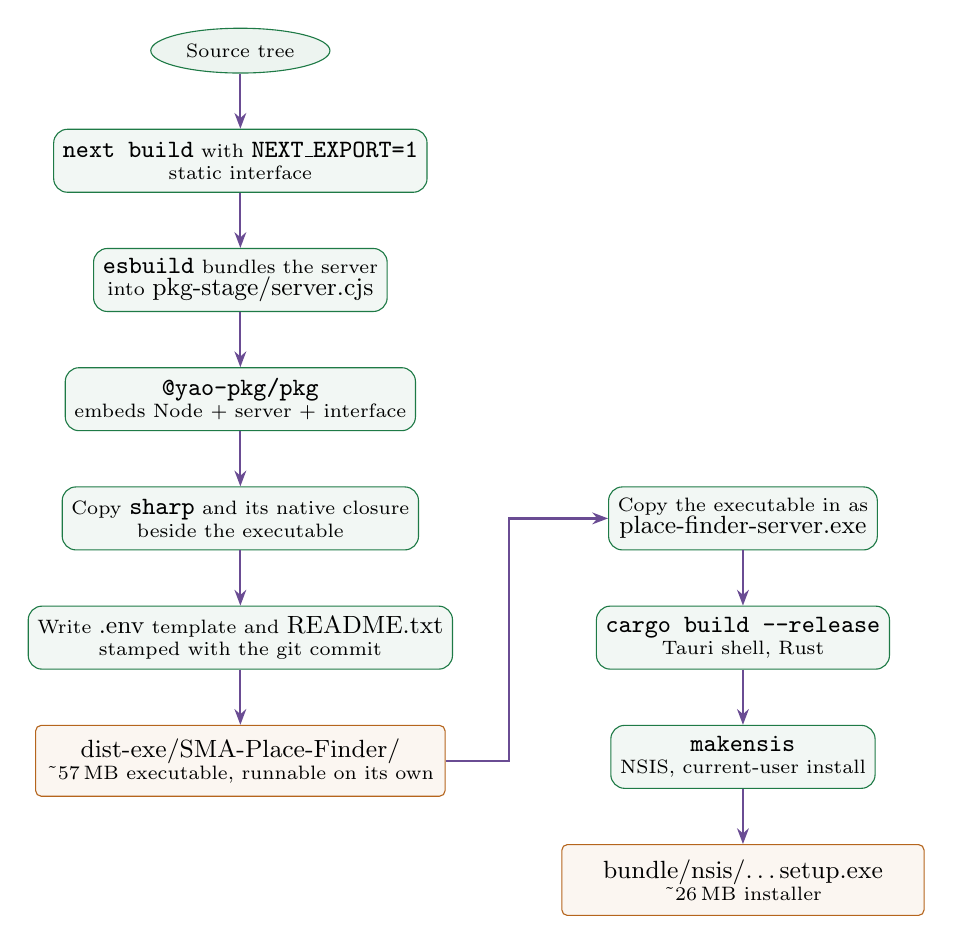
\begin{tikzpicture}[node distance=7mm]
\node[term] (src) {Source tree};
\node[proc, below=of src] (fe) {\code{next build} with \code{NEXT\_EXPORT=1}\\\scriptsize static interface};
\node[proc, below=of fe] (bundle) {\code{esbuild} bundles the server\\\scriptsize into \file{pkg-stage/server.cjs}};
\node[proc, below=of bundle] (pkgs) {\code{@yao-pkg/pkg}\\\scriptsize embeds Node + server + interface};
\node[proc, below=of pkgs] (sharpcp) {Copy \code{sharp} and its native closure\\\scriptsize beside the executable};
\node[proc, below=of sharpcp] (env) {Write \file{.env} template and \file{README.txt}\\\scriptsize stamped with the git commit};
\node[box=cData, below=of env, minimum width=52mm] (exe) {\file{dist-exe/SMA-Place-Finder/}\\\scriptsize \textasciitilde 57\,MB executable, runnable on its own};

\node[proc, right=24mm of sharpcp] (copy) {Copy the executable in as\\\file{place-finder-server.exe}};
\node[proc, below=of copy] (cargo) {\code{cargo build --release}\\\scriptsize Tauri shell, Rust};
\node[proc, below=of cargo] (nsis) {\code{makensis}\\\scriptsize NSIS, current-user install};
\node[box=cData, below=of nsis, minimum width=46mm] (inst) {\file{bundle/nsis/\ldots setup.exe}\\\scriptsize \textasciitilde 26\,MB installer};

\draw[fl=cInfra] (src) -- (fe);
\draw[fl=cInfra] (fe) -- (bundle);
\draw[fl=cInfra] (bundle) -- (pkgs);
\draw[fl=cInfra] (pkgs) -- (sharpcp);
\draw[fl=cInfra] (sharpcp) -- (env);
\draw[fl=cInfra] (env) -- (exe);
\draw[fl=cInfra] (exe.east) -- ++(8mm,0) |- (copy.west);
\draw[fl=cInfra] (copy) -- (cargo);
\draw[fl=cInfra] (cargo) -- (nsis);
\draw[fl=cInfra] (nsis) -- (inst);
\end{tikzpicture}}
\caption[Build and packaging pipeline]{Build and packaging. The installer does
not rebuild the server: it embeds the same executable the standalone edition
ships, so both artefacts contain byte-identical server code.}
\label{fig:build}
\end{figure}

\code{build-exe.mjs} stamps each build with \code{git rev-parse --short HEAD} and
appends \code{-dirty} when \code{git status --porcelain} is non-empty, so a build
made from uncommitted work identifies itself at runtime through
\file{/api/health}.

% =====================================================================
\chapter{Testing Tools}
\label{sec:testing}

\section{What is configured}

\textbf{\code{node:test}} --- the test runner built into Node --- driven by
\code{node --import tsx --test src/**/*.test.mjs}. Assertions use
\code{node:assert/strict}. There is \textbf{no test framework dependency}: no
Jest, Vitest, Mocha, AVA or Jasmine appears in either \file{package.json}.

\begin{longtable}{@{}>{\raggedright\arraybackslash}p{4.4cm}>{\raggedright\arraybackslash}p{10.3cm}@{}}
\caption{Test coverage by area}\label{tab:tests}\\
\toprule
\textbf{Test file} & \textbf{What it covers}\\
\midrule
\endfirsthead
\toprule
\textbf{Test file} & \textbf{What it covers}\\
\midrule
\endhead
\bottomrule
\endfoot
\file{lib/robots.test.mjs}          & robots.txt parsing: group selection, longest-match, wildcards, \code{Crawl-delay}\\
\file{lib/publicUrl.test.mjs}       & SSRF defences: private address ranges, URL vetting\\
\file{lib/connectivity.test.mjs}    & Offline detection and recovery\\
\file{lib/factCheck.test.mjs}       & Stripping unsupported opening-hours claims from generated text\\
\file{lib/llmText.test.mjs}         & Repairing malformed model output\\
\file{lib/travelLinks.test.mjs}     & Outbound deep-link construction\\
\file{services/overpass.test.mjs}   & Selector merging; proves no tag is narrowed away\\
\file{services/siteCrawl.test.mjs}  & Link extraction and scoring; tourism-source catalogue integrity\\
\file{services/hdImages.test.mjs}   & HD threshold and illustrated-place selection\\
\file{services/commonsGateway.test.mjs} & Commons gateway query construction\\
\file{services/folderOutput.test.mjs}& Folder output, no-photo exclusion, non-destructive writes\\
\file{services/fallbackWriteup.test.mjs}& Write-up enrichment from map data; invents nothing when data is absent\\
\file{services/writeup.test.mjs}    & Tolerant parsing of real model output\\
\file{services/batchRecovery.test.mjs}& Batch resume behaviour\\
\end{longtable}

\section{Execution evidence}

The suite was executed while preparing this document, from
\file{backend/}:

\begin{quote}
\code{npm test} $\rightarrow$ \textbf{tests 122, suites 16, pass 122, fail 0}
\end{quote}

Both type checks were also run: \code{npm run typecheck} reports \textbf{zero
errors} across backend and frontend.

\section{What is not configured}

No integration, end-to-end, API, UI or component testing exists: no Playwright,
Cypress, Puppeteer, Supertest or Testing Library. \textbf{No coverage tool} is
configured, so the 122 tests cannot be expressed as a coverage percentage --- they
are unit tests over the library and service functions listed above, and the HTTP
layer, the React components and the Rust shell are untested. There is no static
analysis beyond the TypeScript compiler.

\file{backend/src/eval/} contains \code{harvest.ts} and \code{run.ts}, invoked by
\code{npm run eval}. These are a quality-evaluation harness for search output,
not an automated test suite.

% =====================================================================
\chapter{Deployment Technology and CI/CD}
\label{sec:deploy}

\section{What exists}

\textbf{There is no CI/CD pipeline.} The repository contains no
\file{.github/workflows/}, no GitLab CI, Jenkins, CircleCI or Azure Pipelines
configuration. Nothing builds, tests or releases automatically.

\textbf{There is no container image for the application.} No \file{Dockerfile}
exists anywhere. The single \file{docker-compose.yml} defines \emph{one} service
--- \code{postgres:16-alpine}, with a health check and a named volume --- and is a
convenience for running the optional database locally. It does not deploy this
application.

\textbf{There is no infrastructure-as-code, reverse proxy or web server
configuration} --- no Terraform, Pulumi, Kubernetes manifest, nginx or Apache
configuration, and no platform file for Vercel, Netlify, Railway, Fly or similar.

\section{The actual release process}

Deployment is \textbf{manual packaging and distribution}, performed on a
developer machine:

\begin{enumerate}
\item Commit the work, so the build stamps a clean commit rather than
\code{-dirty}.
\item \code{node build-exe.mjs} --- produces \file{dist-exe/SMA-Place-Finder/}
(OSM edition) and \file{dist-exe/SMA-Place-Finder-Google/}.
\item \code{node build-desktop.mjs} --- embeds that executable and produces the
NSIS installer.
\item Copy the folder, or hand over the installer, to the target machine.
\item Verify by starting it and reading \file{/api/health}, which reports the
build date and commit.
\end{enumerate}

\paragraph{Runtime distribution model.} The product is installed per user
(\code{nsis.installMode: currentUser}) and runs on the operator's own machine.
WebView2 is handled by \code{webviewInstallMode: embedBootstrapper}, so the
installer fetches the runtime if the machine lacks it.

\paragraph{Code signing.} \lblU{} --- no signing configuration or certificate
reference appears in the repository. Unsigned Windows installers raise a
SmartScreen warning on first run.

\section{Health and observability}

\code{GET /api/health} is the only health surface and is used three ways: the
desktop shell polls it to know when the server is ready, the running server uses
it to detect an instance that is already running, and the interface displays its
build stamp. Logging is \code{console} output with bracketed prefixes. There is
\textbf{no structured logging, metrics endpoint, tracing or error-reporting
integration}.

% =====================================================================
\chapter{Hosting Requirements}
\label{sec:hosting}

Each requirement is labelled: \lblV{} established by project files or by
execution; \lblD{} reasonably inferred from the implementation; \lblR{} an
operational suggestion, not a project requirement; \lblU{} insufficient evidence.

\begin{longtable}{@{}>{\raggedright\arraybackslash}p{3.1cm}>{\raggedright\arraybackslash}p{2.6cm}>{\raggedright\arraybackslash}p{9.0cm}@{}}
\caption{Requirements for running the application}\label{tab:hosting}\\
\toprule
\textbf{Requirement} & \textbf{Status} & \textbf{Detail and evidence}\\
\midrule
\endfirsthead
\toprule
\textbf{Requirement} & \textbf{Status} & \textbf{Detail and evidence}\\
\midrule
\endhead
\bottomrule
\endfoot
Operating system (packaged) & \lblV & Windows x64. \code{targets: ["nsis"]}, \code{x86\_64-pc-windows-msvc}, and a PowerShell folder picker\\
Operating system (source)   & \lblD & Backend and frontend are portable Node; only the packaging and the folder picker are Windows-specific\\
Node.js version             & \lblV & \code{engines.node >= 20}; verified running on \ver{v24.18.0}. Not needed for the packaged build --- Node is embedded\\
Rust toolchain              & \lblV & Build-time only. \code{rust-version 1.77.2} declared; \ver{1.98.1} used here\\
WebView2                    & \lblV & Required by the Tauri shell; the installer bootstraps it\\
Disk, installed             & \lblV & \textasciitilde 57\,MB executable, \textasciitilde 26\,MB installer (measured)\\
Disk, output                & \lblD & Grows without bound; the operator chooses the folder. A single place is one PDF plus up to 10 photographs\\
Memory                      & \lblD & Driven by export concurrency: 4 places in flight, each holding its photographs --- on the order of 100\,MB at default settings, plus Node and WebView2\\
CPU                         & \lblU & No measurement exists. The workload is dominated by waiting on remote APIs, not computation\\
Network                     & \lblV & Outbound HTTPS to the services in Figure~\ref{fig:ext} is mandatory; with no connectivity the application detects the outage and waits\\
Inbound ports               & \lblV & TCP 4000 by default, walking upward if occupied; 3000 for the dev interface only. Bound for local use\\
TLS / HTTPS                 & \lblV & Not applicable inbound --- the server is plain HTTP on localhost. All outbound calls are HTTPS\\
Domain / DNS                & \na   & No hosted deployment exists\\
Database                    & \lblV & Optional. Without \code{DATABASE\_URL} an in-memory cache is used; PostgreSQL 16 is what \file{docker-compose.yml} provides\\
Environment variables       & \lblV & All optional with defaults. The packaged build ships a commented \file{.env} beside the executable\\
API keys                    & \lblV & All optional: Flickr, Europeana, Unsplash, Brave, Google Maps, LLM. Absent keys disable that source silently\\
Language model              & \lblV & Optional. Without it, write-ups use the deterministic fallback. Ollama is auto-detected when present\\
Persistent storage          & \lblD & The output folder must persist; nothing else does\\
Logging / monitoring        & \lblR & Only console logging exists. Any retention or alerting would have to be added\\
Backup                      & \lblR & The output folder is the only artefact worth backing up; the caches are disposable\\
Production capacity         & \lblU & \textbf{No load testing has been performed.} No figure for concurrent users or throughput can be given from this repository\\
\end{longtable}

\paragraph{On sizing.} No CPU, RAM or bandwidth figure is stated beyond the
measured artefact sizes and the derived memory behaviour above. The application
has never been load tested, and inventing a server size would be a guess
presented as a requirement. Establishing production capacity requires measuring a
representative batch run on target hardware.

% =====================================================================
\chapter{Important Dependencies and Risk Assessment}
\label{sec:risk}

\begin{longtable}{@{}>{\raggedright\arraybackslash}p{3.2cm}>{\raggedright\arraybackslash}p{2.6cm}>{\raggedright\arraybackslash}p{8.9cm}@{}}
\caption{Operational dependencies and risks}\label{tab:risk}\\
\toprule
\textbf{Area} & \textbf{Severity} & \textbf{Assessment}\\
\midrule
\endfirsthead
\toprule
\textbf{Area} & \textbf{Severity} & \textbf{Assessment}\\
\midrule
\endhead
\bottomrule
\endfoot
Required for startup & --- & \code{express}, \code{cors}, \code{dotenv}, \code{zod}. All small and stable\\
\code{sharp} & Elevated & A native binary that must match the platform. \file{build-exe.mjs} copies it and its closure beside the executable precisely because the bundler cannot embed it. If it fails to load the application still runs, but non-JPEG images are skipped --- the code handles this and says so in the export notes\\
Overpass API & \textbf{High} & The primary source of places, run by volunteers with no availability guarantee. Mitigated in code: three mirrors raced with a hedge, failing mirrors parked for five minutes, and an empty answer never allowed to win\\
Nominatim & \textbf{High} & Geocoding; without it a city cannot be resolved and the search cannot start. Single endpoint, no fallback configured\\
Wikimedia & \textbf{High} & Photographs and research text. Partially mitigated: when \code{commons.wikimedia.org} is unreachable the code falls back to \code{api.wikimedia.org}. Verified behaviour, not theoretical\\
Third-party rate limits & Medium & Public endpoints throttle aggressive use. \file{lib/http.ts} applies per-host pacing; sustained batch runs can still be throttled\\
No authentication & \textbf{High if exposed} & Acceptable while bound to localhost; unacceptable on any reachable interface. See Section~\ref{sec:auth}\\
No CI/CD & Medium & Nothing enforces that tests pass or types check before a build is produced and distributed. The checks exist; running them is manual\\
Unsigned installer & Medium & SmartScreen warns on first run; users must be told to expect it\\
Single-process batch & Medium & One batch job at a time in the API process. Job state is written to disk so a crash can resume, but a crash still interrupts the run\\
\code{pkg} ecosystem & Low--Medium & \code{@yao-pkg/pkg} is a community fork of the discontinued \code{vercel/pkg}. It works here, but the packaging approach depends on that fork continuing\\
Known vulnerabilities & \lblU & \textbf{No audit was run} as part of this document. No claim is made that any dependency is or is not vulnerable. Run \code{npm audit} to establish this\\
Dependency currency & \lblV & Locked versions are recent --- Express 4.22.2, Next 15.5.22, React 19.2.8, TypeScript 5.9.3. Express~4 is the previous major line; Express~5 is released\\
\end{longtable}

\paragraph{Single points of failure.} Three, all external: Nominatim (no
fallback), Overpass (mitigated by mirror racing), and Wikimedia (partially
mitigated by the gateway). Everything internal degrades rather than fails --- a
missing database, a missing LLM, a missing API key and a missing \code{sharp} all
have handled paths.

% =====================================================================
\chapter{Master Technology Stack Table}
\label{sec:master}

Versions are the \emph{locked} versions from \file{package-lock.json} unless
noted. ``Observed'' marks a version measured on the machine used to produce this
document rather than declared by the project.

\begin{longtable}{@{}>{\raggedright\arraybackslash}p{3.0cm}>{\raggedright\arraybackslash}p{4.3cm}>{\raggedright\arraybackslash}p{2.6cm}>{\raggedright\arraybackslash}p{5.2cm}@{}}
\caption{Master technology stack}\label{tab:master}\\
\toprule
\textbf{Category} & \textbf{Technology} & \textbf{Version} & \textbf{Purpose}\\
\midrule
\endfirsthead
\toprule
\textbf{Category} & \textbf{Technology} & \textbf{Version} & \textbf{Purpose}\\
\midrule
\endhead
\bottomrule
\endfoot
Frontend framework   & Next.js                 & \ver{15.5.22} & Interface, dev server, static export\\
UI library           & React                   & \ver{19.2.8}  & Components and hooks\\
                     & React DOM               & \ver{19.2.8}  & DOM rendering\\
Styling              & Tailwind CSS            & \ver{4.3.3}   & All interface styling\\
                     & \code{@tailwindcss/postcss} & \ver{4.3.3} & Build-time Tailwind processing\\
Backend runtime      & Node.js                 & \code{>=20} declared; \ver{24.18.0} observed & Executes the API and all services\\
Backend framework    & Express                 & \ver{4.22.2}  & HTTP routing and middleware\\
Language             & TypeScript              & \ver{5.9.3}   & All application source\\
                     & Rust                    & \code{>=1.77.2} declared; \ver{1.98.1} observed & Desktop shell\\
Desktop shell        & Tauri                   & \ver{2} (major, \file{Cargo.toml}) & Native window and server supervision\\
                     & \code{windows-sys}      & \ver{0.59}    & Job objects, so the server cannot outlive the shell\\
                     & \code{ureq}             & \ver{2}       & Health polling from the shell\\
Validation           & Zod                     & \ver{3.25.76} & Request schemas\\
PDF generation       & PDFKit                  & \ver{0.15.2}  & Per-place and summary PDFs\\
Image processing     & sharp                   & \ver{0.33.5}  & JPEG conversion and re-encoding\\
Archiving            & archiver                & \ver{7.0.1}   & ZIP for browser downloads\\
HTTP middleware      & cors                    & \ver{2.8.6}   & Cross-origin access for the dev interface\\
Configuration        & dotenv                  & \ver{16.6.1}  & Loads the \file{.env} beside the executable\\
Database (optional)  & PostgreSQL              & \ver{16} & Optional shared search cache; image \code{postgres:16-alpine}\\
Database driver      & \code{pg}               & \ver{8.22.0}  & Client, loaded only when configured\\
Default storage      & In-memory store         & \na           & Search cache; the default\\
Authentication       & \textbf{None implemented} & \na         & No identity or access control exists\\
API style            & REST over HTTP, JSON    & \na           & Client--server communication\\
Build tool           & esbuild                 & \ver{0.28.1}  & Server bundling before packaging\\
                     & \code{@yao-pkg/pkg}     & \ver{6.22.0}  & Single-file executable\\
                     & Next.js bundler         & \ver{15.5.22} & Interface build and static export\\
Dev runner           & tsx                     & \ver{4.23.5}  & Runs TypeScript directly\\
Package manager      & npm                     & \ver{11.16.0} observed; lockfile v3 & Dependency management\\
Testing              & \code{node:test}        & Node built-in & 122 unit tests, 16 suites, all passing\\
Installer            & NSIS via Tauri bundler  & \nv           & Windows installer, current-user\\
CI/CD                & \textbf{None}           & \na           & No automated pipeline exists\\
Containerisation     & Docker Compose (database only) & \nv    & Local PostgreSQL convenience only\\
Hosting              & Local desktop           & \na           & No hosted deployment exists\\
\end{longtable}

% =====================================================================
\chapter{Technology Interaction Matrix}
\label{sec:matrix}

\begin{longtable}{@{}>{\raggedright\arraybackslash}p{3.0cm}>{\raggedright\arraybackslash}p{3.0cm}>{\raggedright\arraybackslash}p{2.6cm}>{\raggedright\arraybackslash}p{3.0cm}>{\raggedright\arraybackslash}p{3.2cm}@{}}
\caption{How the components communicate}\label{tab:matrix}\\
\toprule
\textbf{Source} & \textbf{Target} & \textbf{Method} & \textbf{Purpose} & \textbf{Evidence}\\
\midrule
\endfirsthead
\toprule
\textbf{Source} & \textbf{Target} & \textbf{Method} & \textbf{Purpose} & \textbf{Evidence}\\
\midrule
\endhead
\bottomrule
\endfoot
Next.js interface & Express API & HTTP/JSON \code{fetch} & All operations & \file{frontend/lib/api.ts}\\
Interface & \file{/api/search/progress/:id} & HTTP polling & Live search progress & \file{SearchProgress.tsx}\\
Interface & \file{/api/batch/:jobId} & HTTP polling & Batch job state & \file{BatchPanel.tsx}\\
Interface & openstreetmap.org & \code{<iframe>} embed & Map display & \file{MapView.tsx}\\
Tauri shell & Packaged server & Child process + TCP & Starts it, polls \file{/api/health} & \file{desktop/src-tauri/src/main.rs}\\
Tauri shell & Windows kernel & Job object API & Server cannot outlive the window & \code{windows-sys}, \file{main.rs}\\
Express routes & Services & In-process calls & Business logic & \file{routes/}, \file{services/}\\
Services & Overpass mirrors & HTTPS POST & Place discovery & \file{services/overpass.ts}\\
Services & Nominatim & HTTPS GET & Geocoding & \file{services/geocode.ts}\\
Services & Wikidata / Wikipedia / Wikivoyage & HTTPS GET & Research text and facts & \file{services/content.ts}\\
Services & Commons, \code{api.wikimedia.org} & HTTPS GET & Photographs, with gateway fallback & \file{services/images.ts}\\
Services & Flickr, Europeana, Unsplash, Brave & HTTPS GET & Extra photographs, when keyed & \file{services/imageSources.ts}\\
Services & Official tourism sites & HTTPS GET, robots-respecting & Write-up material & \file{services/siteCrawl.ts}\\
Services & LLM endpoint & HTTPS POST, OpenAI-compatible & Filtering, translation, articles & \file{services/llm.ts}\\
Services & Search cache & In-process or SQL & Result reuse between search and export & \file{services/cache.ts}\\
\code{cache.ts} & PostgreSQL & TCP 5432 via \code{pg} & Optional shared cache & \file{services/cache.ts}\\
\code{archive.ts} & Filesystem & \code{fs} writes & The output folder & \file{services/archive.ts}\\
\code{batch.ts} & PowerShell & \code{execFile} & Native folder picker & \file{routes/batch.ts}\\
\end{longtable}

% =====================================================================
\chapter{Repository Evidence and Verification Notes}
\label{sec:evidence}

\section{Files inspected}

\begin{longtable}{@{}>{\raggedright\arraybackslash}p{6.0cm}>{\raggedright\arraybackslash}p{8.7cm}@{}}
\caption{Primary evidence}\label{tab:evidence}\\
\toprule
\textbf{File} & \textbf{What it established}\\
\midrule
\endfirsthead
\toprule
\textbf{File} & \textbf{What it established}\\
\midrule
\endhead
\bottomrule
\endfoot
\file{package.json} (root)            & Workspace scripts; npm with \code{--prefix}\\
\file{backend/package.json}           & Runtime and dev dependencies; \code{engines.node}; test command\\
\file{backend/package-lock.json}      & Locked backend versions (lockfile v3)\\
\file{frontend/package.json}          & Next, React, Tailwind; absence of state and UI libraries\\
\file{frontend/package-lock.json}     & Locked frontend versions\\
\file{backend/tsconfig.json}          & \code{ES2022}, \code{NodeNext}, \code{strict}\\
\file{frontend/tsconfig.json}         & \code{ES2022}, \code{esnext}, \code{strict}\\
\file{backend/src/index.ts}           & Middleware order, routers, static serving, port selection\\
\file{backend/src/config.ts}          & All settings, defaults, limits, external endpoints\\
\file{backend/src/routes/*.ts}        & Endpoint inventory, Zod validation, rate limits\\
\file{backend/src/services/cache.ts}  & Storage strategy and the PostgreSQL fallback\\
\file{backend/src/services/archive.ts}& Output structure, folder/ZIP sinks, photo gate\\
\file{backend/src/services/overpass.ts}& Mirror racing, health memory, selector merging\\
\file{frontend/next.config.mjs}       & Static export switch; permitted remote image hosts\\
\file{frontend/postcss.config.mjs}    & Tailwind~4 via PostCSS\\
\file{frontend/app/globals.css}       & CSS-first Tailwind configuration\\
\file{frontend/lib/api.ts}            & API base URL and the polling model\\
\file{desktop/src-tauri/Cargo.toml}   & Rust edition, \code{rust-version}, Tauri and \code{windows-sys}\\
\file{desktop/src-tauri/tauri.conf.json}& Bundle targets, resources, WebView2, install mode\\
\file{build-exe.mjs}                  & Packaging pipeline, \file{.env} template, build stamping\\
\file{build-desktop.mjs}              & Installer pipeline and server embedding\\
\file{docker-compose.yml}             & PostgreSQL 16 service; absence of an application image\\
\end{longtable}

\section{How versions were established}

\begin{itemize}
\item \textbf{npm packages} --- read from the \code{packages} map of each
\file{package-lock.json}, not from the declared ranges in \file{package.json}.
Both are shown in Section~\ref{sec:libs} so the difference is visible.
\item \textbf{Node and npm} --- \code{node --version} and \code{npm --version} on
the machine used here, labelled ``observed''. The project only declares
\code{>=20}.
\item \textbf{Rust} --- \code{rustc --version} observed; \file{Cargo.toml}
declares the minimum.
\item \textbf{Tauri, ureq, windows-sys} --- major versions from
\file{Cargo.toml}. \textbf{\file{Cargo.lock} was not consulted}, so exact
resolved crate versions are \nv{}.
\item \textbf{PostgreSQL} --- the image tag \code{postgres:16-alpine}.
\end{itemize}

\section{Limitations and open questions}

\begin{itemize}
\item \textbf{No design rationale exists.} There is no architecture decision
record. Every ``why'' in Chapter~\ref{sec:why} is an interpretation of observed
use.
\item \textbf{Exact Rust crate versions} were not resolved from
\file{Cargo.lock}.
\item \textbf{No dependency audit} was performed; no vulnerability claim is made
either way.
\item \textbf{No coverage measurement} exists, so the 122 passing tests cannot be
expressed as a proportion of the code.
\item \textbf{No load testing} exists, so no capacity figure is given.
\item \textbf{The \code{lint} script is not runnable} as written --- \code{next
lint} is defined but ESLint is neither configured nor installed.
\item \textbf{The Google edition} is built from the same source with
\code{PLACE\_SOURCE=google}; its behaviour was not exercised while preparing this
document.
\end{itemize}

% =====================================================================
\chapter{Final Summary}
\label{sec:summary}

\section{The confirmed stack}

A TypeScript application, end to end. An \textbf{Express} API on \textbf{Node.js}
does all the work; a \textbf{Next.js}/\textbf{React} interface with
\textbf{Tailwind} styling drives it; a \textbf{Tauri} shell in \textbf{Rust}
presents it as a Windows desktop program. Documents are produced with
\textbf{PDFKit}, images normalised with \textbf{sharp}, archives written with
\textbf{archiver}, and every request validated with \textbf{Zod}. Tests run on
Node's own runner --- 122 of them, all passing.

\section{Architectural characteristics that matter}

\begin{enumerate}
\item \textbf{Local-first.} No hosted component. Each deployment is a copy
running on someone's machine, which is why there is no authentication and why
that is defensible.
\item \textbf{Orchestration, not computation.} The substance is coordinating a
dozen public APIs. Availability and rate limits of those services dominate
behaviour far more than local resources.
\item \textbf{Degradation over failure.} Missing database, missing LLM, missing
API key, blocked Commons host, failed \code{sharp} load, lost connectivity --- each
has a handled path. The application narrows what it produces instead of
refusing to run.
\item \textbf{The filesystem is the product.} Caches are disposable; the output
folder is the artefact.
\item \textbf{A deliberately small dependency surface.} Eleven direct runtime
dependencies across both halves, no framework for testing, state, UI components
or data access.
\end{enumerate}

\section{What could not be established}

Exact Rust crate versions; dependency vulnerability status; test coverage;
production capacity; and the original rationale for any technology choice.

\section{Recommended next steps}

These are suggestions, not findings. Nothing below is a defect in the current
product.

\begin{enumerate}
\item \textbf{Add continuous integration.} The checks already exist
(\code{npm test}, \code{npm run typecheck}); nothing enforces them before a
build is distributed. This is the cheapest meaningful improvement available.
\item \textbf{Run \code{npm audit}} and record the result, so dependency risk is
known rather than unlabelled.
\item \textbf{Make the \code{lint} script real} --- install and configure ESLint,
or remove the script so it does not imply a check that cannot run.
\item \textbf{Add authentication before any network exposure.} Only necessary if
the deployment model changes; today it would be unnecessary complexity.
\item \textbf{Consider code signing} to remove the SmartScreen warning.
\item \textbf{Measure a representative batch run} on target hardware to replace
the \lblU{} capacity entries in Table~\ref{tab:hosting} with figures.
\item \textbf{Record a short architecture decision log}, so future readers inherit
the reasoning this document had to infer.
\end{enumerate}

\vspace{1em}
\noindent\rule{\textwidth}{0.4pt}\\
\footnotesize
\textit{Every technology, version and component above was read from the
repository at commit \code{cfb509b}. Items that could not be verified are marked
\nv{}, \lblU{} or stated as absent. No credentials or secret values appear in
this document.}

\end{document}
